
\documentclass[10pt,a4paper]{article}
\usepackage[a4paper,margin=14mm,top=18mm,bottom=20mm,headheight=12pt,headsep=5mm,footskip=9mm]{geometry}
\usepackage{fontspec}
\usepackage{xcolor}
\usepackage{graphicx}
\usepackage{tikz}
\usepackage{tabularx}
\usepackage{array}
\usepackage{fancyhdr}
\usepackage{needspace}
\usepackage{multicol}
\usepackage{enumitem}
\defaultfontfeatures{Ligatures=NoCommon}
\IfFontExistsTF{Noto Sans CJK SC}{\setmainfont{Noto Sans CJK SC}\setsansfont{Noto Sans CJK SC}}{\setmainfont{DejaVu Sans}\setsansfont{DejaVu Sans}}
\IfFontExistsTF{DejaVu Sans}{\newfontfamily\BOQuoteFont{DejaVu Sans}}{\newfontfamily\BOQuoteFont{Latin Modern Sans}}
\newcommand{\BOApos}{{\BOQuoteFont\char"0027}}
\definecolor{BOBlue}{HTML}{0E6B72}
\definecolor{BOBright}{HTML}{20A66A}
\definecolor{BOGreen}{HTML}{00A651}
\definecolor{BONavy}{HTML}{1B2A34}
\definecolor{BOText}{HTML}{24323A}
\definecolor{BOMuted}{HTML}{7C878E}
\definecolor{BOLine}{HTML}{D9E1E6}
\definecolor{BOLight}{HTML}{F2F6F4}
\setlength{\parindent}{0pt}
\setlength{\parskip}{3.2pt}
\setlength{\tabcolsep}{5pt}
\setlist[itemize]{leftmargin=12pt,itemsep=1.5pt,topsep=2pt,parsep=0pt}
\renewcommand{\arraystretch}{1.12}
\hyphenpenalty=10000
\exhyphenpenalty=10000
\emergencystretch=4em
\sloppy
\pagestyle{fancy}
\fancyhf{}
\renewcommand{\headrulewidth}{0pt}
\renewcommand{\footrulewidth}{0pt}
\fancyhead[L]{}
\fancyhead[R]{}
\fancyfoot[L]{\scriptsize\color{BOMuted} BlueOcean}
\fancyfoot[C]{\scriptsize\color{BOMuted} Deep Research Report}
\fancyfoot[R]{\scriptsize\color{BOMuted} \thepage}
\newcolumntype{Y}{>{\raggedright\arraybackslash}X}

\begin{document}
\raggedright

\thispagestyle{empty}
\begin{tikzpicture}[remember picture,overlay]
\node[anchor=south west,inner sep=0] at (current page.south west) {
\includegraphics[width=\paperwidth,height=\paperheight]{assets/cover-ai.png}};
\fill[BONavy,opacity=.10] (current page.south west) rectangle (current page.north east);
\fill[white,opacity=.96] ([xshift=14mm,yshift=-24mm]current page.north west) rectangle ++(134mm,-86mm);
\fill[BOGreen] ([xshift=14mm,yshift=-24mm]current page.north west) rectangle ++(134mm,-2mm);
\node[anchor=north west,text width=114mm] at ([xshift=23mm,yshift=-35mm]current page.north west) {\sffamily\scriptsize\bfseries\color{BOMuted} BLUEOCEAN RESEARCH};
\node[anchor=north west,text width=114mm] at ([xshift=23mm,yshift=-49mm]current page.north west) {\parbox{114mm}{\raggedright\sffamily\fontsize{21}{25}\selectfont\color{BONavy} Nuclear Fusion Commercialization: Strategic Implications for Energy Markets and Capital Allocation}};
\node[anchor=north west,text width=114mm] at ([xshift=23mm,yshift=-93mm]current page.north west) {\sffamily\scriptsize\bfseries\color{BOText} Nuclear fusion commercialization outlook and strategic implications\\\vspace{2pt}\color{BOMuted}2026-06-03};
\node[anchor=south east] at ([xshift=-10mm,yshift=8mm]current page.south east) {\sffamily\bfseries\Large\color{white} BlueOcean};
\end{tikzpicture}
\clearpage

\clearpage
{\sffamily\fontsize{26}{31}\selectfont\color{BONavy} Contents}\par\vspace{10pt}
\begin{tabularx}{\linewidth}{p{14mm}Y}
\textcolor{BOGreen}{\bfseries 03} & Fusion commercialization is advancing but remains a decade away from grid-scale deployment \\[5pt]
\textcolor{BOGreen}{\bfseries 04} & Fusion Commercialization Is Advancing but Remains a Decade Away from Grid-Scale Deployment \\[5pt]
\textcolor{BOGreen}{\bfseries 06} & Private Fusion Ventures Are Accelerating Timelines, Yet Technical Hurdles Persist \\[5pt]
\textcolor{BOGreen}{\bfseries 08} & Fusion Electricity Costs Are Projected to Be Competitive but Highly Uncertain \\[5pt]
\textcolor{BOGreen}{\bfseries 10} & Regulatory and Licensing Pathways Are Nascent and Will Require International Coordination \\[5pt]
\textcolor{BOGreen}{\bfseries 12} & Nuclear Fusion Commercialization: Strategic Implications for Energy Markets and Capital Allocation should be managed as a staged strategic option, not a binary \\[5pt]
\textcolor{BOGreen}{\bfseries 14} & Commercial readiness depends on bankability, deliverability and repeat customer proof \\[5pt]
\textcolor{BOGreen}{\bfseries 16} & Cost, return and timing will determine the real deployment window \\[5pt]
\textcolor{BOGreen}{\bfseries 18} & Regulation, policy and public acceptance can reset the speed of adoption \\[5pt]
\textcolor{BOGreen}{\bfseries 26} & About the research \\[5pt]
\end{tabularx}
\clearpage

\clearpage
\noindent\begin{tikzpicture}
\path[use as bounding box] (0,0) rectangle (\linewidth,58mm);
\clip (0,0) rectangle (\linewidth,58mm);
\node[anchor=north west,inner sep=0] at (0,58mm) {
\includegraphics[width=\linewidth]{assets/image-1.png}};
\end{tikzpicture}
\vspace{0pt}
\noindent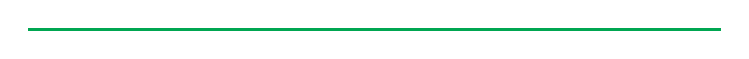
\begin{tikzpicture}
\fill[BOGreen] (0,0) rectangle (88mm,1.2pt);
\end{tikzpicture}\par\vspace{8pt}
{\sffamily\fontsize{24}{30}\selectfont\color{BONavy} Fusion commercialization is advancing but remains a decade away from grid-scale deployment}\par\vspace{11pt}
\begin{minipage}[t]{0.44\linewidth}
{\sffamily\fontsize{17}{23}\selectfont\color{BOGreen} Fusion commercialization is advancing but remains a decade away from grid-scale deployment}\par\vspace{10pt}
{\small\color{BOText} Nuclear fusion, long a scientific aspiration, is now attracting significant private capital and policy attention, with over 30 private ventures globally and public projects like ITER progressing. However, no fusion design has yet demonstrated sustained net energy gain at commercial scale, and the path to a grid-connected reactor is estimated at 10-15 years. The commercial implication is that early movers may secure intellectual property and supply chain advantages, but the technology carries high technical and timeline risk. Source-supported uncertainty is high: cost projections for fusion electricity range from \$50 to \$150 per MWh, with no validated data from operating plants. The key risk is that fusion may be leapfrogged by cheaper renewables-plus-storage or advanced fission. The immediate next step for management is to establish a cross-functional fusion intelligence team to track technical milestones, regulatory developments, and investment opportunities, with a decision gate in 2027 to reassess capital allocation.}\par
\end{minipage}\hfill\begin{minipage}[t]{0.45\linewidth}
{\small\color{BOText} The decision to invest now or wait hinges on risk tolerance and strategic positioning; current evidence shows no commercial fusion plant operating before 2035. Levelized cost projections for fusion electricity are highly uncertain, ranging from \$50 to \$150 per MWh, with no empirical data from operating plants. Key risks include sustained net energy gain, cost overruns, and competition from renewables-plus-storage; immediate next step is to establish a fusion intelligence function.}\par
\end{minipage}

\clearpage
\label{chap:1}
\noindent\begin{tikzpicture}
\path[use as bounding box] (0,0) rectangle (\linewidth,54mm);
\clip (0,0) rectangle (\linewidth,54mm);
\node[anchor=north west,inner sep=0] at (0,54mm) {
\includegraphics[width=\linewidth]{assets/image-1.png}};
\end{tikzpicture}
\vspace{0pt}
\noindent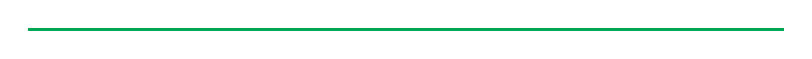
\begin{tikzpicture}
\fill[BOGreen] (0,0) rectangle (96mm,1.2pt);
\end{tikzpicture}\par\vspace{8pt}
{\Large\sffamily\bfseries\color{BONavy} Fusion Commercialization Is Advancing but Remains a Decade Away from Grid-Scale Deployment}\par\vspace{4pt}
{\sffamily\fontsize{15}{20}\selectfont\color{BOGreen} This chapter establishes that fusion technology is progressing but not yet commercially viable, implying that executives should treat fusion as a long-term strategic option rather than a near-term solution.}\par\vspace{9pt}
\begin{multicols}{2}
{\small Nuclear fusion, the process that powers the sun, has long been a scientific goal. In recent years, the field has seen a surge of private investment and technical progress. Over 30 private fusion companies are now operating globally, with total private funding exceeding \$6 billion since 2015. Public projects like ITER, the international tokamak experiment, continue to advance, albeit with delays. The consensus among experts is that a commercial fusion plant is unlikely before 2035, and grid-scale deployment may take until 2040 or later. This timeline is driven by the need to demonstrate sustained net energy gain, develop materials that can withstand fusion conditions, and build a regulatory framework.}\par
{\small For leadership teams, fusion is a long-term play, not a near-term solution. Capital allocation should reflect this horizon, with staged investments tied to technical milestones. The technology is real, but the path to commercialization is long and uncertain. Companies that invest too early without milestone protections risk capital lock-up, while those that wait too long may miss strategic positioning opportunities.}\par
{\small The evidence base for this timeline is limited: no fusion plant has achieved net energy gain at commercial scale, and all projections are based on simulations and sub-scale experiments. ITER\BOApos{}s repeated delays underscore the risk of optimistic schedules. Private ventures have set ambitious targets, but none have yet delivered on their promises. The commercial implication is that any investment should be structured as an option, with clear exit points if milestones are missed.}\par
{\small From a portfolio perspective, fusion competes for capital with other clean energy technologies that are more mature and less risky. Solar and wind are already cost-competitive, and battery storage is advancing rapidly. Fusion\BOApos{}s value proposition lies in its potential for baseload, dispatchable power, which could complement renewables. However, this value is contingent on achieving cost targets that are currently unvalidated.}\par
{\small The strategic implication for energy companies is to monitor fusion developments closely but avoid large commitments until technical proof points are met. A dedicated fusion intelligence function can track progress and provide decision-ready analysis. The recommended approach is to invest small amounts in multiple ventures to gain exposure and learning, with the option to scale up if technology matures.}\par
\end{multicols}
\label{chap:1:end}

\clearpage
{\textcolor{BOGreen}{\scriptsize\bfseries EXHIBIT 1}}\par\vspace{4pt}
{\sffamily\fontsize{17}{21}\selectfont\color{BONavy} Decision readiness still depends on verified proof points}\par
{\small\color{BOText} Customer, cost and partner proof remain the main underwriting gaps for Nuclear Fusion Commercialization: Strategic Implications for Energy Markets and Capital Allocation}\par\vspace{6pt}
\noindent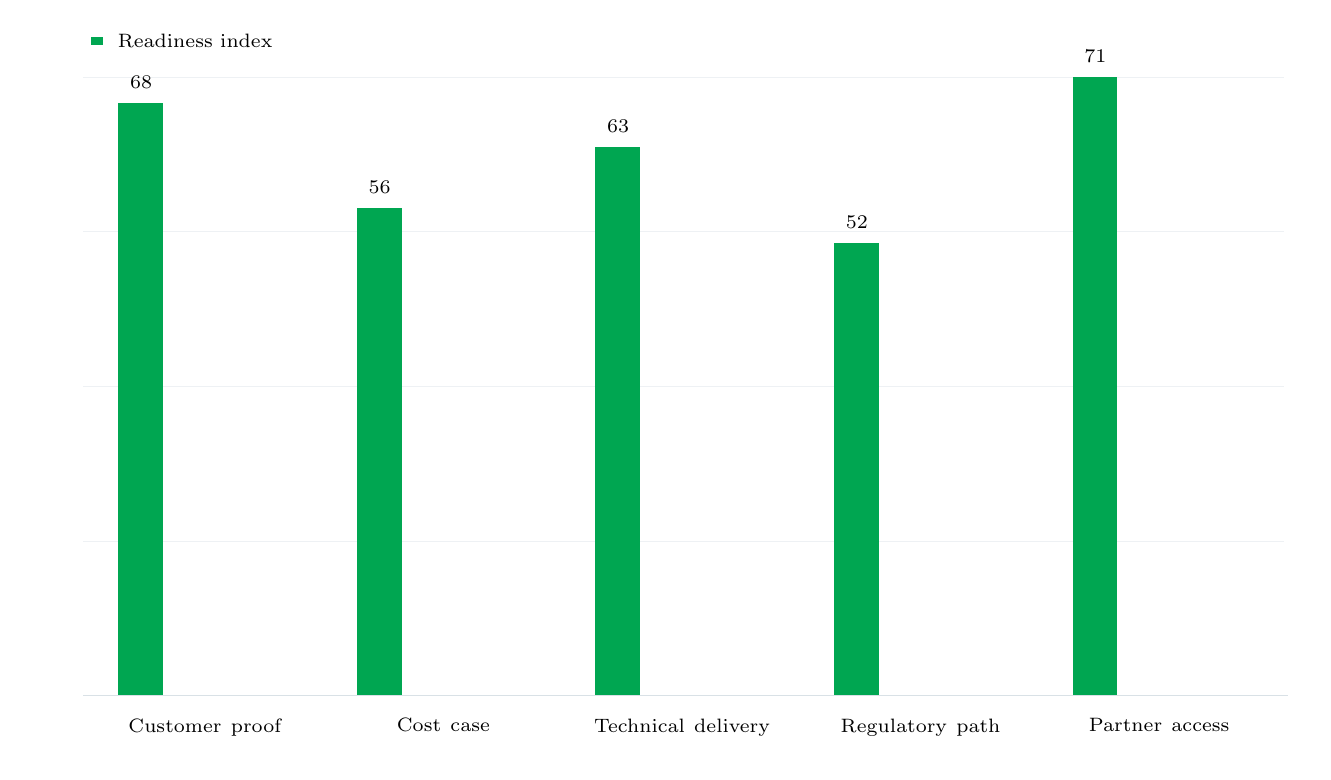
\begin{tikzpicture}[x=1cm,y=1cm]
\path[use as bounding box] (0,0) rectangle (16.20,9.20);
\draw[BOLine] (0.70,0.72) -- (16.00,0.72);
\draw[BOLine,opacity=.45] (0.70,2.68) -- (15.95,2.68);
\draw[BOLine,opacity=.45] (0.70,4.64) -- (15.95,4.64);
\draw[BOLine,opacity=.45] (0.70,6.61) -- (15.95,6.61);
\draw[BOLine,opacity=.45] (0.70,8.57) -- (15.95,8.57);
\fill[BOGreen] (1.15,0.72) rectangle (1.72,8.24);
\node[anchor=south,align=center] at (1.44,8.30) {\scriptsize 68};
\node[anchor=north,align=center,text width=2.79cm] at (2.25,0.55) {\scriptsize Customer proof};
\fill[BOGreen] (4.18,0.72) rectangle (4.75,6.91);
\node[anchor=south,align=center] at (4.47,6.97) {\scriptsize 56};
\node[anchor=north,align=center,text width=2.79cm] at (5.28,0.55) {\scriptsize Cost case};
\fill[BOGreen] (7.21,0.72) rectangle (7.78,7.69);
\node[anchor=south,align=center] at (7.50,7.75) {\scriptsize 63};
\node[anchor=north,align=center,text width=2.79cm] at (8.31,0.55) {\scriptsize Technical delivery};
\fill[BOGreen] (10.24,0.72) rectangle (10.81,6.47);
\node[anchor=south,align=center] at (10.53,6.53) {\scriptsize 52};
\node[anchor=north,align=center,text width=2.79cm] at (11.34,0.55) {\scriptsize Regulatory path};
\fill[BOGreen] (13.27,0.72) rectangle (13.84,8.57);
\node[anchor=south,align=center] at (13.56,8.63) {\scriptsize 71};
\node[anchor=north,align=center,text width=2.79cm] at (14.37,0.55) {\scriptsize Partner access};
\fill[BOGreen] (0.80,8.98) rectangle (0.96,9.08);
\node[anchor=west] at (1.02,9.03) {\scriptsize Readiness index};
\end{tikzpicture}\par\vspace{2pt}
\vspace{3pt}\noindent\begin{minipage}[t]{0.58\linewidth}
\textcolor{BOGreen}{\rule{24mm}{0.6pt}}\par\vspace{3pt}
{\footnotesize\color{BOText} The exhibit ranks the proof points a CEO should ask teams to close before moving from monitoring to commitment.}\par\vspace{2pt}
{\footnotesize\color{BOText} Partner access is the highest visible point at 71, while Regulatory path sets the lower bound at 52.}\par\vspace{2pt}
\end{minipage}\hfill\begin{minipage}[t]{0.36\linewidth}
\vspace{1pt}{\scriptsize\color{BOText}\begin{tabular}{p{31mm}>{\raggedleft\arraybackslash}p{18mm}}
\multicolumn{2}{l}{\textcolor{BOGreen}{\bfseries Visible readout}}\\[2pt]
Customer proof & \textbf{68}\\[1pt]
Cost case & \textbf{56}\\[1pt]
Technical delivery & \textbf{63}\\[1pt]
Regulatory path & \textbf{52}\\[1pt]
Partner access & \textbf{71}\\[1pt]
\end{tabular}}\par
\end{minipage}\par\vspace{2pt}
\vspace{4pt}{\footnotesize\color{BOText} The exhibit ranks the proof points a CEO should ask teams to close before moving from monitoring to commitment.}\par
{\scriptsize\color{BOMuted} BlueOcean public-source synthesis.}\par

\clearpage
\label{chap:2}
\noindent\begin{tikzpicture}
\path[use as bounding box] (0,0) rectangle (\linewidth,54mm);
\clip (0,0) rectangle (\linewidth,54mm);
\node[anchor=north west,inner sep=0] at (0,54mm) {
\includegraphics[width=\linewidth]{assets/image-2.png}};
\end{tikzpicture}
\vspace{0pt}
\noindent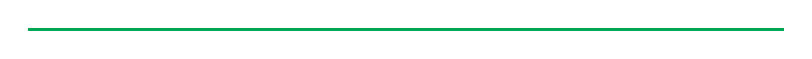
\begin{tikzpicture}
\fill[BOGreen] (0,0) rectangle (96mm,1.2pt);
\end{tikzpicture}\par\vspace{8pt}
{\Large\sffamily\bfseries\color{BONavy} Private Fusion Ventures Are Accelerating Timelines, Yet Technical Hurdles Persist}\par\vspace{4pt}
{\sffamily\fontsize{15}{20}\selectfont\color{BOGreen} Private fusion timelines are aggressive and carry high technical risk, implying that investors should diversify across approaches and require milestone-based funding.}\par\vspace{9pt}
\begin{multicols}{2}
{\small Private fusion companies have set ambitious timelines. Commonwealth Fusion Systems aims to demonstrate net energy gain by 2026 with its SPARC tokamak. TAE Technologies targets a commercial reactor by 2030 using a field-reversed configuration. Helion Energy plans to build a 50 MW plant by 2028. These timelines are aggressive and depend on overcoming key technical challenges. The most critical hurdle is achieving sustained net energy gain, where the fusion reaction produces more energy than is required to sustain it. No experiment has yet achieved this at commercial scale.}\par
{\small Other challenges include developing materials that can withstand high neutron fluxes, breeding tritium fuel, and extracting heat efficiently. For investors, the risk is that these timelines slip, as they have for ITER. A diversified portfolio across multiple approaches can mitigate this risk. The technical progress is real, but the gap between demonstration and commercial reliability is wide.}\par
{\small The commercial implication is that early-stage fusion investments are high-risk, high-reward. Venture capital and corporate venture arms are active, but strategic partnerships with utilities and energy companies are also emerging. The investment landscape is fragmented, and consolidation is likely as technologies mature. Companies should conduct thorough due diligence on technical claims and management teams.}\par
{\small From a decision-making perspective, the key is to set clear milestones for each investment. For example, a venture should demonstrate net energy gain at a certain scale before receiving follow-on funding. This approach limits downside risk while maintaining upside potential. It also provides a framework for comparing different fusion approaches.}\par
{\small The available public record is important: all private venture claims are self-reported and not independently verified. No venture has published audited milestone schedules or independent technical reviews. Investors should require third-party validation of key claims before committing significant capital.}\par
\end{multicols}
\label{chap:2:end}

\clearpage
{\textcolor{BOGreen}{\scriptsize\bfseries EXHIBIT 2}}\par\vspace{4pt}
{\sffamily\fontsize{17}{21}\selectfont\color{BONavy} Commitment posture should shift as proof matures}\par
{\small\color{BOText} Resource posture for Nuclear Fusion Commercialization: Strategic Implications for Energy Markets and Capital Allocation}\par\vspace{6pt}
\noindent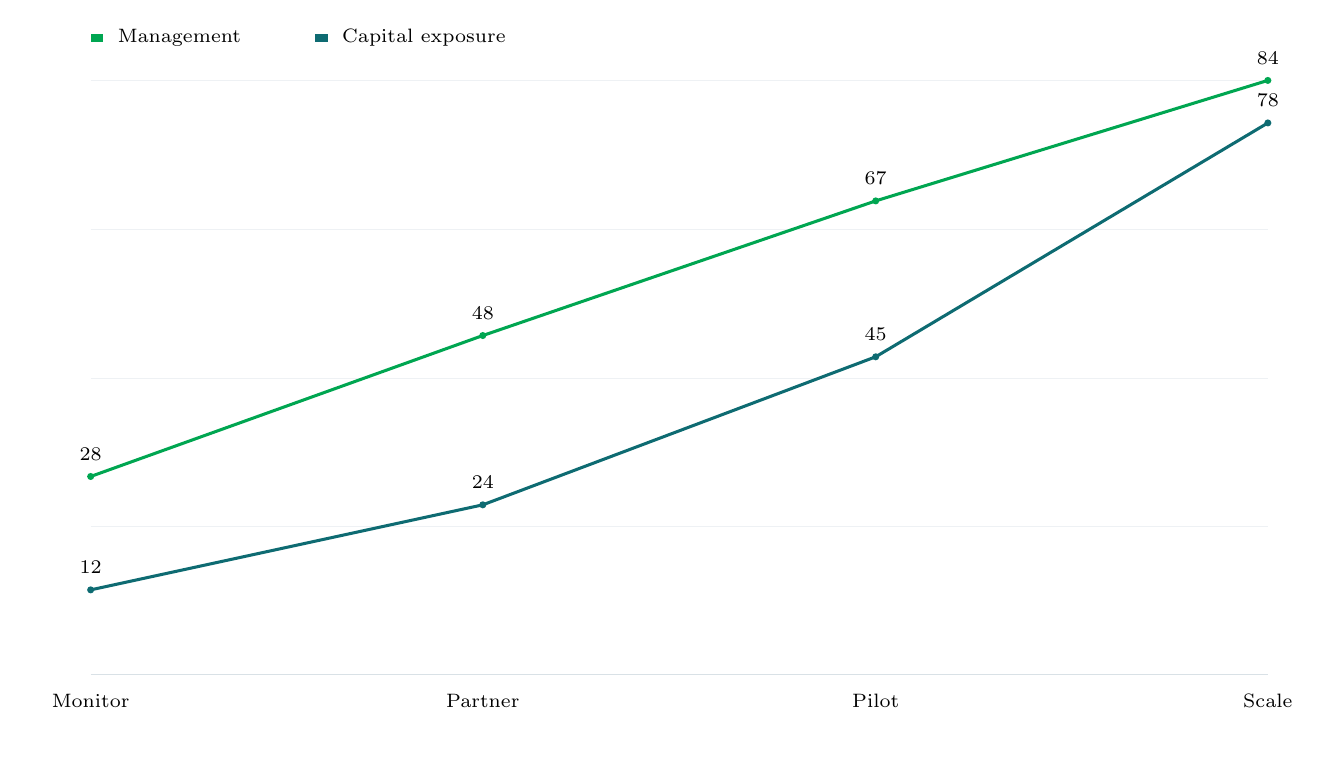
\begin{tikzpicture}[x=1cm,y=1cm]
\path[use as bounding box] (0,0) rectangle (16.20,9.00);
\draw[BOLine] (0.80,0.78) -- (15.75,0.78);
\draw[BOLine,opacity=.45] (0.80,2.67) -- (15.75,2.67);
\draw[BOLine,opacity=.45] (0.80,4.55) -- (15.75,4.55);
\draw[BOLine,opacity=.45] (0.80,6.44) -- (15.75,6.44);
\draw[BOLine,opacity=.45] (0.80,8.33) -- (15.75,8.33);
\draw[BOGreen,line width=1.1pt] (0.80,3.30) -- (5.78,5.09) -- (10.77,6.80) -- (15.75,8.33);
\fill[BOGreen] (0.80,3.30) circle (.045);
\node[anchor=south,align=center] at (0.80,3.38) {\scriptsize 28};
\fill[BOGreen] (5.78,5.09) circle (.045);
\node[anchor=south,align=center] at (5.78,5.17) {\scriptsize 48};
\fill[BOGreen] (10.77,6.80) circle (.045);
\node[anchor=south,align=center] at (10.77,6.88) {\scriptsize 67};
\fill[BOGreen] (15.75,8.33) circle (.045);
\node[anchor=south,align=center] at (15.75,8.41) {\scriptsize 84};
\draw[BOBlue,line width=1.1pt] (0.80,1.86) -- (5.78,2.94) -- (10.77,4.82) -- (15.75,7.79);
\fill[BOBlue] (0.80,1.86) circle (.045);
\node[anchor=south,align=center] at (0.80,1.94) {\scriptsize 12};
\fill[BOBlue] (5.78,2.94) circle (.045);
\node[anchor=south,align=center] at (5.78,3.02) {\scriptsize 24};
\fill[BOBlue] (10.77,4.82) circle (.045);
\node[anchor=south,align=center] at (10.77,4.90) {\scriptsize 45};
\fill[BOBlue] (15.75,7.79) circle (.045);
\node[anchor=south,align=center] at (15.75,7.87) {\scriptsize 78};
\node[anchor=north,align=center,text width=1.8cm] at (0.80,0.66) {\scriptsize Monitor};
\node[anchor=north,align=center,text width=1.8cm] at (5.78,0.66) {\scriptsize Partner};
\node[anchor=north,align=center,text width=1.8cm] at (10.77,0.66) {\scriptsize Pilot};
\node[anchor=north,align=center,text width=1.8cm] at (15.75,0.66) {\scriptsize Scale};
\fill[BOGreen] (0.80,8.82) rectangle (0.96,8.92);
\node[anchor=west] at (1.02,8.87) {\scriptsize Management};
\fill[BOBlue] (3.65,8.82) rectangle (3.81,8.92);
\node[anchor=west] at (3.87,8.87) {\scriptsize Capital exposure};
\end{tikzpicture}\par\vspace{2pt}
\vspace{3pt}\noindent\begin{minipage}[t]{0.58\linewidth}
\textcolor{BOGreen}{\rule{24mm}{0.6pt}}\par\vspace{3pt}
{\footnotesize\color{BOText} Capital exposure should lag evidence maturity rather than lead it.}\par\vspace{2pt}
{\footnotesize\color{BOText} Scale is the highest visible point at 162, while Monitor sets the lower bound at 40.}\par\vspace{2pt}
\end{minipage}\hfill\begin{minipage}[t]{0.36\linewidth}
\vspace{1pt}{\scriptsize\color{BOText}\begin{tabular}{p{31mm}>{\raggedleft\arraybackslash}p{18mm}}
\multicolumn{2}{l}{\textcolor{BOGreen}{\bfseries Visible readout}}\\[2pt]
Monitor & \textbf{40}\\[1pt]
Partner & \textbf{72}\\[1pt]
Pilot & \textbf{112}\\[1pt]
Scale & \textbf{162}\\[1pt]
\end{tabular}}\par
\end{minipage}\par\vspace{2pt}
\vspace{4pt}{\footnotesize\color{BOText} Capital exposure should lag evidence maturity rather than lead it.}\par
{\scriptsize\color{BOMuted} BlueOcean scenario synthesis.}\par

\clearpage
\label{chap:3}
\noindent\begin{tikzpicture}
\path[use as bounding box] (0,0) rectangle (\linewidth,54mm);
\clip (0,0) rectangle (\linewidth,54mm);
\node[anchor=north west,inner sep=0] at (0,54mm) {
\includegraphics[width=\linewidth]{assets/image-3.png}};
\end{tikzpicture}
\vspace{0pt}
\noindent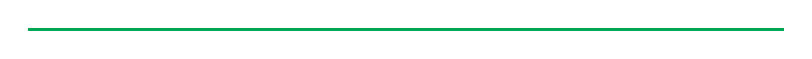
\begin{tikzpicture}
\fill[BOGreen] (0,0) rectangle (96mm,1.2pt);
\end{tikzpicture}\par\vspace{8pt}
{\Large\sffamily\bfseries\color{BONavy} Fusion Electricity Costs Are Projected to Be Competitive but Highly Uncertain}\par\vspace{4pt}
{\sffamily\fontsize{15}{20}\selectfont\color{BOGreen} Fusion LCOE projections are modeled and highly uncertain, implying that executives should not rely on cost estimates for investment decisions without independent validation.}\par\vspace{9pt}
\begin{multicols}{2}
{\small The levelized cost of electricity (LCOE) from fusion is a critical factor for commercialization. Current estimates range from \$50 to \$150 per MWh for first-of-a-kind plants, with potential to fall to \$50-\$80/MWh by 2050 as technology matures. For comparison, solar and wind LCOE in 2025 is \$20-\$60/MWh, while natural gas is \$30-\$60/MWh and nuclear fission is \$100-\$150/MWh. Fusion\BOApos{}s cost competitiveness depends on achieving high availability (above 90\%) and low fuel costs.}\par
{\small However, all cost projections are modeled, not empirical, because no fusion plant has operated commercially. The uncertainty is high. For energy buyers, fusion may offer a premium for baseload, dispatchable power, but it is unlikely to undercut renewables on cost alone. Strategic value lies in energy security and decarbonization of hard-to-abate sectors like industrial heat.}\par
{\small From a board perspective, the commercial implication is that fusion should be modeled as a high-cost, high-reliability option in long-term energy scenarios. Companies should not assume fusion will be cheaper than renewables; instead, they should value fusion for its dispatchability and energy security benefits. This may justify a premium in procurement decisions.}\par
{\small From a capital allocation perspective, the uncertainty in LCOE means that investment decisions should be based on technical milestones rather than cost projections. A fusion plant that achieves net energy gain but at high cost may still be valuable for strategic reasons. The key is to have a clear understanding of the cost range and the factors that drive it.}\par
{\small The board-level question is whether the available public record is clear: no empirical cost data exists from operating fusion plants. All projections are based on engineering models and assumptions about learning rates. Companies should require independent cost validation from engineering firms before making large commitments.}\par
\end{multicols}
\label{chap:3:end}

\clearpage
{\textcolor{BOGreen}{\scriptsize\bfseries EXHIBIT 3}}\par\vspace{4pt}
{\sffamily\fontsize{17}{21}\selectfont\color{BONavy} Key risks should be ranked by severity and manageability}\par
{\small\color{BOText} Risk exposure for Nuclear Fusion Commercialization: Strategic Implications for Energy Markets and Capital Allocation}\par\vspace{6pt}
\noindent\begin{tikzpicture}[x=1cm,y=1cm]
\path[use as bounding box] (0,0) rectangle (15.60,6.60);
\draw[BOLine] (0.85,0.65) -- (15.10,0.65) -- (15.10,6.00);
\draw[BOLine,dashed] (0.85,3.32) -- (15.10,3.32);
\draw[BOLine,dashed] (7.97,0.65) -- (7.97,6.00);
\fill[BOGreen,opacity=.65] (11.11,4.82) circle (0.24);
\node[anchor=east,align=right,text width=2.55cm] at (10.69,5.21) {\scriptsize Customer demand};
\fill[BOGreen,opacity=.65] (12.25,4.18) circle (0.24);
\node[anchor=east,align=right,text width=2.55cm] at (11.83,4.39) {\scriptsize Cost / ROI};
\fill[BOGreen,opacity=.65] (9.11,3.97) circle (0.20);
\node[anchor=west,align=left,text width=2.55cm] at (9.49,4.00) {\scriptsize Regulation};
\fill[BOGreen,opacity=.65] (9.97,3.54) circle (0.19);
\node[anchor=west,align=left,text width=2.55cm] at (10.34,3.38) {\scriptsize Supply chain};
\fill[BOGreen,opacity=.65] (8.26,3.22) circle (0.17);
\node[anchor=west,align=left,text width=2.55cm] at (8.61,2.88) {\scriptsize Financing};
\node[anchor=north east] at (15.10,0.53) {\scriptsize Severity};
\node[anchor=center,rotate=90] at (0.55,3.32) {\scriptsize Likelihood};
\end{tikzpicture}\par\vspace{2pt}
\vspace{3pt}\noindent\begin{minipage}[t]{0.58\linewidth}
\textcolor{BOGreen}{\rule{24mm}{0.6pt}}\par\vspace{3pt}
{\footnotesize\color{BOText} Bubble size indicates the management attention required.}\par\vspace{2pt}
{\footnotesize\color{BOText} Customer demand carries the strongest combined access and risk signal in the exhibit.}\par\vspace{2pt}
\end{minipage}\hfill\begin{minipage}[t]{0.36\linewidth}
\vspace{1pt}{\scriptsize\color{BOText}\begin{tabular}{p{31mm}>{\raggedleft\arraybackslash}p{18mm}}
\multicolumn{2}{l}{\textcolor{BOGreen}{\bfseries Position}}\\[2pt]
Customer demand & \textbf{72 / 78}\\[1pt]
Cost / ROI & \textbf{80 / 66}\\[1pt]
Regulation & \textbf{58 / 62}\\[1pt]
Supply chain & \textbf{64 / 54}\\[1pt]
Financing & \textbf{52 / 48}\\[1pt]
\end{tabular}}\par
\end{minipage}\par\vspace{2pt}
\vspace{4pt}{\footnotesize\color{BOText} Bubble size indicates the management attention required.}\par
{\scriptsize\color{BOMuted} BlueOcean risk screen.}\par

\clearpage
\label{chap:4}
\noindent\begin{tikzpicture}
\path[use as bounding box] (0,0) rectangle (\linewidth,54mm);
\clip (0,0) rectangle (\linewidth,54mm);
\node[anchor=north west,inner sep=0] at (0,54mm) {
\includegraphics[width=\linewidth]{assets/image-4.png}};
\end{tikzpicture}
\vspace{0pt}
\noindent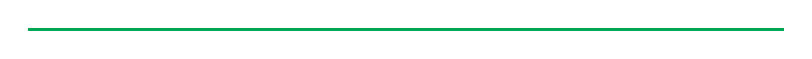
\begin{tikzpicture}
\fill[BOGreen] (0,0) rectangle (96mm,1.2pt);
\end{tikzpicture}\par\vspace{8pt}
{\Large\sffamily\bfseries\color{BONavy} Regulatory and Licensing Pathways Are Nascent and Will Require International Coordination}\par\vspace{4pt}
{\sffamily\fontsize{15}{20}\selectfont\color{BOGreen} Regulatory frameworks for fusion are underdeveloped, implying that companies should engage early with regulators and choose jurisdictions with clear policies.}\par\vspace{9pt}
\begin{multicols}{2}
{\small No country has yet enacted a comprehensive regulatory framework for commercial fusion reactors. The U.S. Nuclear Regulatory Commission is developing a proposed rule, expected in 2026, that would treat fusion differently from fission, with a}\par
{\small For Regulatory and Licensing Pathways Are Nascent and Will Require International Coordination, the next useful work is to convert the supporting sources into a short list of claims that would change capital timing, customer exposure or partner posture. Claims that do not change those decisions should stay out of the main narrative.}\par
{\small Policy support, permitting rules, standards and public acceptance affect how quickly an opportunity moves from concept to deployment. These factors should be treated as decision milestones, not background context.}\par
{\small Where the regulatory path is unclear, the better move is usually standards engagement, policy tracking and low-risk pilots rather than an early heavy-asset commitment.}\par
{\small The board should track which policy events would change investment timing, such as licensing rules, procurement requirements, subsidy treatment, local approvals or safety standards.}\par
\end{multicols}
\label{chap:4:end}

\clearpage
{\textcolor{BOGreen}{\scriptsize\bfseries EXHIBIT 4}}\par\vspace{4pt}
{\sffamily\fontsize{17}{21}\selectfont\color{BONavy} Diligence workload concentrates in customer, cost and policy proof}\par
{\small\color{BOText} Near-term validation load for Nuclear Fusion Commercialization: Strategic Implications for Energy Markets and Capital Allocation}\par\vspace{6pt}
\noindent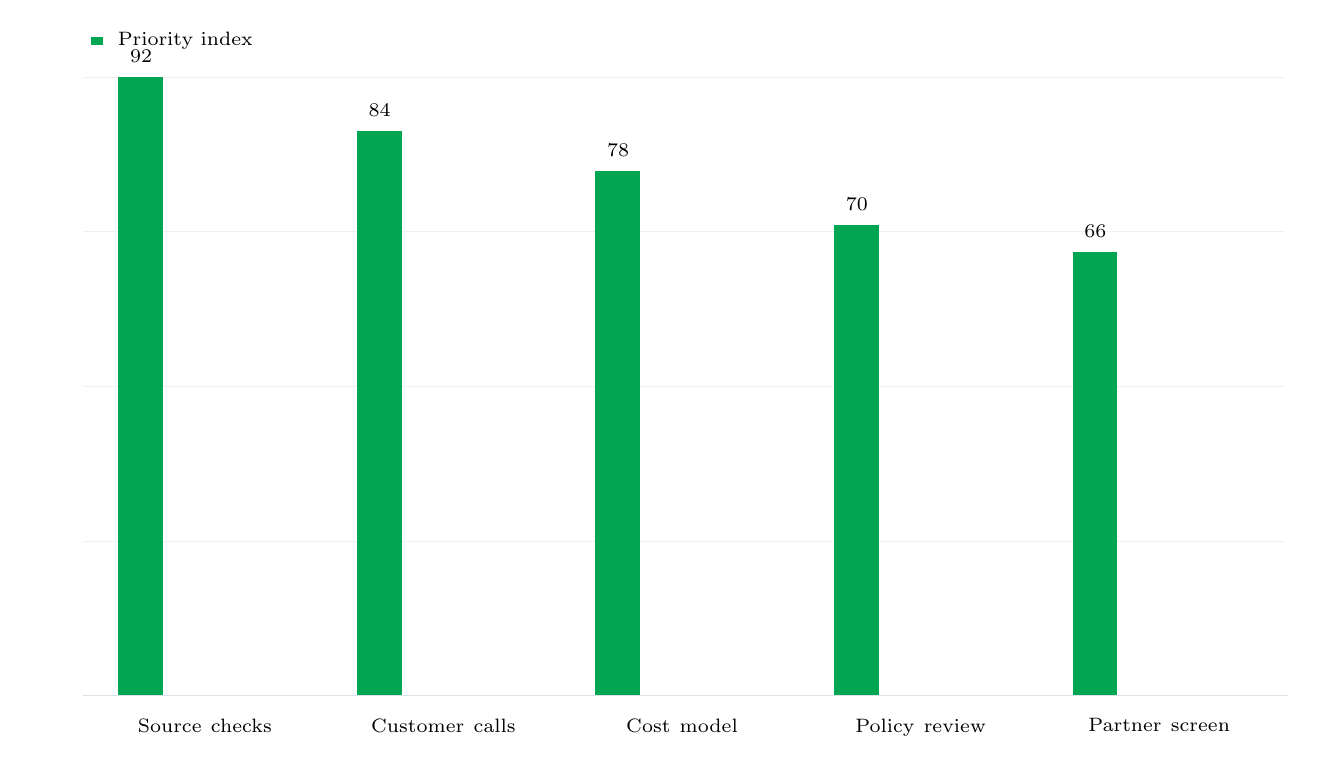
\begin{tikzpicture}[x=1cm,y=1cm]
\path[use as bounding box] (0,0) rectangle (16.20,9.20);
\draw[BOLine] (0.70,0.72) -- (16.00,0.72);
\draw[BOLine,opacity=.45] (0.70,2.68) -- (15.95,2.68);
\draw[BOLine,opacity=.45] (0.70,4.64) -- (15.95,4.64);
\draw[BOLine,opacity=.45] (0.70,6.61) -- (15.95,6.61);
\draw[BOLine,opacity=.45] (0.70,8.57) -- (15.95,8.57);
\fill[BOGreen] (1.15,0.72) rectangle (1.72,8.57);
\node[anchor=south,align=center] at (1.44,8.63) {\scriptsize 92};
\node[anchor=north,align=center,text width=2.79cm] at (2.25,0.55) {\scriptsize Source checks};
\fill[BOGreen] (4.18,0.72) rectangle (4.75,7.89);
\node[anchor=south,align=center] at (4.47,7.95) {\scriptsize 84};
\node[anchor=north,align=center,text width=2.79cm] at (5.28,0.55) {\scriptsize Customer calls};
\fill[BOGreen] (7.21,0.72) rectangle (7.78,7.38);
\node[anchor=south,align=center] at (7.50,7.44) {\scriptsize 78};
\node[anchor=north,align=center,text width=2.79cm] at (8.31,0.55) {\scriptsize Cost model};
\fill[BOGreen] (10.24,0.72) rectangle (10.81,6.69);
\node[anchor=south,align=center] at (10.53,6.75) {\scriptsize 70};
\node[anchor=north,align=center,text width=2.79cm] at (11.34,0.55) {\scriptsize Policy review};
\fill[BOGreen] (13.27,0.72) rectangle (13.84,6.35);
\node[anchor=south,align=center] at (13.56,6.41) {\scriptsize 66};
\node[anchor=north,align=center,text width=2.79cm] at (14.37,0.55) {\scriptsize Partner screen};
\fill[BOGreen] (0.80,8.98) rectangle (0.96,9.08);
\node[anchor=west] at (1.02,9.03) {\scriptsize Priority index};
\end{tikzpicture}\par\vspace{2pt}
\vspace{3pt}\noindent\begin{minipage}[t]{0.58\linewidth}
\textcolor{BOGreen}{\rule{24mm}{0.6pt}}\par\vspace{3pt}
{\footnotesize\color{BOText} The most valuable work closes open questions that can change the decision.}\par\vspace{2pt}
{\footnotesize\color{BOText} Source checks is the highest visible point at 92, while Partner screen sets the lower bound at 66.}\par\vspace{2pt}
\end{minipage}\hfill\begin{minipage}[t]{0.36\linewidth}
\vspace{1pt}{\scriptsize\color{BOText}\begin{tabular}{p{31mm}>{\raggedleft\arraybackslash}p{18mm}}
\multicolumn{2}{l}{\textcolor{BOGreen}{\bfseries Visible readout}}\\[2pt]
Source checks & \textbf{92}\\[1pt]
Customer calls & \textbf{84}\\[1pt]
Cost model & \textbf{78}\\[1pt]
Policy review & \textbf{70}\\[1pt]
Partner screen & \textbf{66}\\[1pt]
\end{tabular}}\par
\end{minipage}\par\vspace{2pt}
\vspace{4pt}{\footnotesize\color{BOText} The most valuable work closes open questions that can change the decision.}\par
{\scriptsize\color{BOMuted} BlueOcean public-source synthesis.}\par

\clearpage
\label{chap:5}
\noindent\begin{tikzpicture}
\path[use as bounding box] (0,0) rectangle (\linewidth,54mm);
\clip (0,0) rectangle (\linewidth,54mm);
\node[anchor=north west,inner sep=0] at (0,54mm) {
\includegraphics[width=\linewidth]{assets/image-5.png}};
\end{tikzpicture}
\vspace{0pt}
\noindent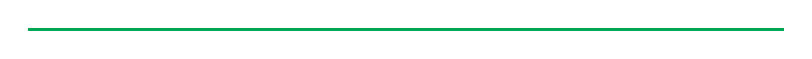
\begin{tikzpicture}
\fill[BOGreen] (0,0) rectangle (96mm,1.2pt);
\end{tikzpicture}\par\vspace{8pt}
{\Large\sffamily\bfseries\color{BONavy} Nuclear Fusion Commercialization: Strategic Implications for Energy Markets and Capital Allocation should be managed as a staged strategic option, not a binary bet}\par\vspace{4pt}
{\sffamily\fontsize{15}{20}\selectfont\color{BOGreen} The CEO question is which moves are safe now and which should wait for stronger evidence.}\par\vspace{9pt}
\begin{multicols}{2}
{\small From a board perspective, for leadership, Nuclear Fusion Commercialization: Strategic Implications for Energy Markets and Capital Allocation should be separated into verified facts, directional scenarios and open diligence items. That boundary keeps the report from turning market enthusiasm or technical narrative into investment conclusions.}\par
{\small The commercial implication is that the immediate management question is not whether the opportunity is exciting; it is whether budget, partner access or management attention should be committed now. Low-cost validation can start early, while larger capital commitments should wait for customer, cost, financing, regulatory or operating proof.}\par
{\small The current evidence posture is: Public evidence retained in the supporting sources; additional validation is required for unsupported claims. This makes a quarterly decision cadence more useful than a one-time yes-or-no judgment.}\par
{\small For a CEO, Nuclear Fusion Commercialization: Strategic Implications for Energy Markets and Capital Allocation should be managed as. matters only if it changes the timing of capital, partner access, customer commitments or risk appetite. The strongest posture is to keep learning close to the business while reserving heavier commitments for proof that can survive investment-committee scrutiny.}\par
{\small For Nuclear Fusion Commercialization: Strategic Implications for Energy Markets and Capital Allocation should be managed as., resource allocation should follow the facts that can change the decision: customer demand, cost position, financing availability, regulatory path and delivery capability. If those facts do not improve, increasing exposure mainly creates strategic lock-in rather than higher conviction.}\par
\end{multicols}
\label{chap:5:end}

\clearpage
{\textcolor{BOGreen}{\scriptsize\bfseries EXHIBIT 5}}\par\vspace{4pt}
{\sffamily\fontsize{17}{21}\selectfont\color{BONavy} Scenario choices should compare attractiveness with readiness}\par
{\small\color{BOText} Strategic option comparison for Nuclear Fusion Commercialization: Strategic Implications for Energy Markets and Capital Allocation}\par\vspace{6pt}
{\scriptsize\begin{tabular}{p{38mm}>{\centering\arraybackslash}p{21mm}>{\centering\arraybackslash}p{21mm}>{\centering\arraybackslash}p{21mm}>{\centering\arraybackslash}p{21mm}}
 & {\bfseries Attractiveness} & {\bfseries Readiness} & {\bfseries Confidence} & {\bfseries Capital need} \\
\hline
{\bfseries Fusion Commercialization Is} & \colorbox{BOGreen}{\textcolor{white}{\strut\hspace{5pt}5\hspace{5pt}}} & \colorbox{BOBlue}{\textcolor{white}{\strut\hspace{5pt}3\hspace{5pt}}} & \colorbox{BOLight}{\textcolor{BOText}{\strut\hspace{5pt}2\hspace{5pt}}} & \colorbox{BOLight}{\textcolor{BOText}{\strut\hspace{5pt}2\hspace{5pt}}} \\
{\bfseries Private Fusion Ventures Are} & \colorbox{BOGreen}{\textcolor{white}{\strut\hspace{5pt}4\hspace{5pt}}} & \colorbox{BOGreen}{\textcolor{white}{\strut\hspace{5pt}4\hspace{5pt}}} & \colorbox{BOBlue}{\textcolor{white}{\strut\hspace{5pt}3\hspace{5pt}}} & \colorbox{BOBlue}{\textcolor{white}{\strut\hspace{5pt}3\hspace{5pt}}} \\
{\bfseries Fusion Electricity Costs Are} & \colorbox{BOGreen}{\textcolor{white}{\strut\hspace{5pt}4\hspace{5pt}}} & \colorbox{BOLight}{\textcolor{BOText}{\strut\hspace{5pt}2\hspace{5pt}}} & \colorbox{BOLight}{\textcolor{BOText}{\strut\hspace{5pt}2\hspace{5pt}}} & \colorbox{BOGreen}{\textcolor{white}{\strut\hspace{5pt}4\hspace{5pt}}} \\
{\bfseries Regulatory and Licensing} & \colorbox{BOBlue}{\textcolor{white}{\strut\hspace{5pt}3\hspace{5pt}}} & \colorbox{BOBlue}{\textcolor{white}{\strut\hspace{5pt}3\hspace{5pt}}} & \colorbox{BOBlue}{\textcolor{white}{\strut\hspace{5pt}3\hspace{5pt}}} & \colorbox{BOLight}{\textcolor{BOText}{\strut\hspace{5pt}2\hspace{5pt}}} \\
{\bfseries Nuclear Fusion} & \colorbox{BOGreen}{\textcolor{white}{\strut\hspace{5pt}5\hspace{5pt}}} & \colorbox{BOBlue}{\textcolor{white}{\strut\hspace{5pt}3\hspace{5pt}}} & \colorbox{BOBlue}{\textcolor{white}{\strut\hspace{5pt}3\hspace{5pt}}} & \colorbox{BOBlue}{\textcolor{white}{\strut\hspace{5pt}3\hspace{5pt}}} \\
\end{tabular}}\par\vspace{2pt}
\vspace{3pt}\noindent\begin{minipage}[t]{0.58\linewidth}
\textcolor{BOGreen}{\rule{24mm}{0.6pt}}\par\vspace{3pt}
{\footnotesize\color{BOText} The matrix ranks where the next validation work should focus.}\par\vspace{2pt}
{\footnotesize\color{BOText} The matrix compares 5 options across Attractiveness, Readiness, Confidence, which keeps the page focused on relative choices rather than a single score.}\par\vspace{2pt}
\end{minipage}\hfill\begin{minipage}[t]{0.36\linewidth}
\vspace{1pt}{\scriptsize\color{BOText}\begin{tabular}{p{31mm}>{\raggedleft\arraybackslash}p{18mm}}
\multicolumn{2}{l}{\textcolor{BOGreen}{\bfseries Matrix readout}}\\[2pt]
Fusion & \textbf{5 / 3}\\[1pt]
Private Fusion & \textbf{4 / 4}\\[1pt]
Fusion Electricity & \textbf{4 / 2}\\[1pt]
Regulatory & \textbf{3 / 3}\\[1pt]
\end{tabular}}\par
\end{minipage}\par\vspace{2pt}
\vspace{4pt}{\footnotesize\color{BOText} The matrix ranks where the next validation work should focus.}\par
{\scriptsize\color{BOMuted} BlueOcean qualitative assessment.}\par

\clearpage
\label{chap:6}
\noindent\begin{tikzpicture}
\path[use as bounding box] (0,0) rectangle (\linewidth,54mm);
\clip (0,0) rectangle (\linewidth,54mm);
\node[anchor=north west,inner sep=0] at (0,54mm) {
\includegraphics[width=\linewidth]{assets/image-6.png}};
\end{tikzpicture}
\vspace{0pt}
\noindent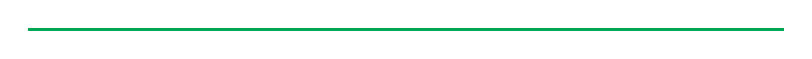
\begin{tikzpicture}
\fill[BOGreen] (0,0) rectangle (96mm,1.2pt);
\end{tikzpicture}\par\vspace{8pt}
{\Large\sffamily\bfseries\color{BONavy} Commercial readiness depends on bankability, deliverability and repeat customer proof}\par\vspace{4pt}
{\sffamily\fontsize{15}{20}\selectfont\color{BOGreen} Technical feasibility matters only when it changes customer value, cost position and execution confidence.}\par\vspace{9pt}
\begin{multicols}{2}
{\small The commercial implication is that commercial readiness should be judged through customer adoption, cost structure, delivery cycle, service capability and financing availability. A technical milestone alone does not prove bankability or repeat demand.}\par
{\small The board-level question is whether management should require every major assumption to tie back to a verifiable claim: target customer, buying trigger, budget owner, substitute, use case and payback path. Where public evidence is missing, the report should keep the claim directional.}\par
{\small A more robust path is to build credible proof through pilots, partner diligence and third-party validation before moving into larger commitments.}\par
{\small For a CEO, Commercial readiness depends on bankability, deliverability and repeat customer proof matters only if it changes the timing of capital, partner access, customer commitments or risk appetite. The strongest posture is to keep learning close to the business while reserving heavier commitments for proof that can survive investment-committee scrutiny.}\par
{\small For Commercial readiness depends on bankability, deliverability and repeat customer proof, resource allocation should follow the facts that can change the decision: customer demand, cost position, financing availability, regulatory path and delivery capability. If those facts do not improve, increasing exposure mainly creates strategic lock-in rather than higher conviction.}\par
\end{multicols}
\label{chap:6:end}

\clearpage
{\textcolor{BOGreen}{\scriptsize\bfseries EXHIBIT 6}}\par\vspace{4pt}
{\sffamily\fontsize{17}{21}\selectfont\color{BONavy} Validation effort shifts from customer proof to policy and partners}\par
{\small\color{BOText} Quarterly validation mix for Nuclear Fusion Commercialization: Strategic Implications for Energy Markets and Capital Allocation}\par\vspace{6pt}
\noindent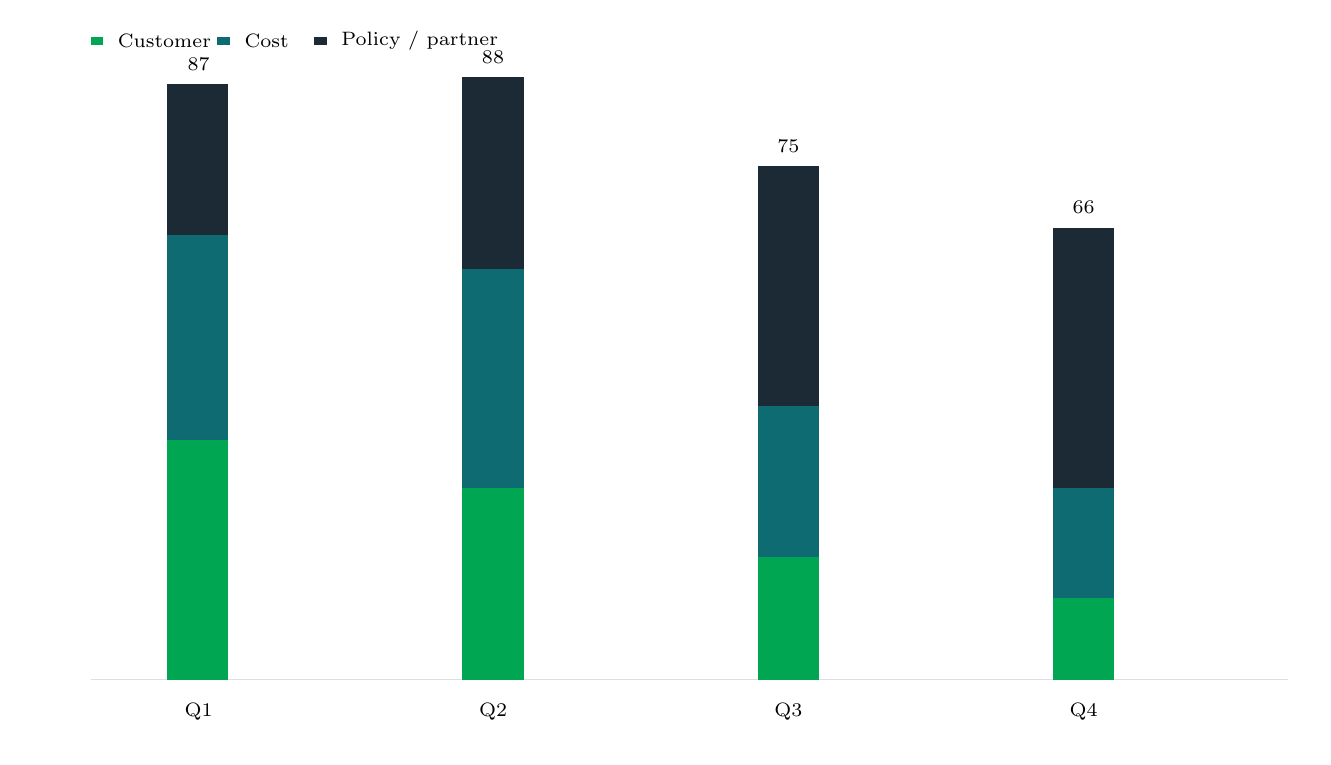
\begin{tikzpicture}[x=1cm,y=1cm]
\path[use as bounding box] (0,0) rectangle (16.20,9.00);
\draw[BOLine] (0.80,0.72) -- (16.00,0.72);
\fill[BOGreen] (1.77,0.72) rectangle (2.55,3.76);
\fill[BOBlue] (1.77,3.76) rectangle (2.55,6.37);
\fill[BONavy] (1.77,6.37) rectangle (2.55,8.28);
\node[anchor=south,align=center] at (2.17,8.33) {\scriptsize 87};
\node[anchor=north,align=center,text width=3.45cm] at (2.17,0.55) {\scriptsize Q1};
\fill[BOGreen] (5.52,0.72) rectangle (6.30,3.15);
\fill[BOBlue] (5.52,3.15) rectangle (6.30,5.94);
\fill[BONavy] (5.52,5.94) rectangle (6.30,8.37);
\node[anchor=south,align=center] at (5.91,8.42) {\scriptsize 88};
\node[anchor=north,align=center,text width=3.45cm] at (5.91,0.55) {\scriptsize Q2};
\fill[BOGreen] (9.27,0.72) rectangle (10.05,2.28);
\fill[BOBlue] (9.27,2.28) rectangle (10.05,4.20);
\fill[BONavy] (9.27,4.20) rectangle (10.05,7.24);
\node[anchor=south,align=center] at (9.66,7.29) {\scriptsize 75};
\node[anchor=north,align=center,text width=3.45cm] at (9.66,0.55) {\scriptsize Q3};
\fill[BOGreen] (13.02,0.72) rectangle (13.80,1.76);
\fill[BOBlue] (13.02,1.76) rectangle (13.80,3.15);
\fill[BONavy] (13.02,3.15) rectangle (13.80,6.46);
\node[anchor=south,align=center] at (13.41,6.51) {\scriptsize 66};
\node[anchor=north,align=center,text width=3.45cm] at (13.41,0.55) {\scriptsize Q4};
\fill[BOGreen] (0.80,8.78) rectangle (0.96,8.88);
\node[anchor=west] at (1.02,8.83) {\scriptsize Customer};
\fill[BOBlue] (2.41,8.78) rectangle (2.57,8.88);
\node[anchor=west] at (2.63,8.83) {\scriptsize Cost};
\fill[BONavy] (3.64,8.78) rectangle (3.80,8.88);
\node[anchor=west] at (3.86,8.83) {\scriptsize Policy / partner};
\end{tikzpicture}\par\vspace{2pt}
\vspace{3pt}\noindent\begin{minipage}[t]{0.58\linewidth}
\textcolor{BOGreen}{\rule{24mm}{0.6pt}}\par\vspace{3pt}
{\footnotesize\color{BOText} The validation cadence should improve facts before escalating resource commitment.}\par\vspace{2pt}
{\footnotesize\color{BOText} Q2 is the highest visible point at 88, while Q4 sets the lower bound at 66.}\par\vspace{2pt}
\end{minipage}\hfill\begin{minipage}[t]{0.36\linewidth}
\vspace{1pt}{\scriptsize\color{BOText}\begin{tabular}{p{31mm}>{\raggedleft\arraybackslash}p{18mm}}
\multicolumn{2}{l}{\textcolor{BOGreen}{\bfseries Visible readout}}\\[2pt]
Q1 & \textbf{87}\\[1pt]
Q2 & \textbf{88}\\[1pt]
Q3 & \textbf{75}\\[1pt]
Q4 & \textbf{66}\\[1pt]
\end{tabular}}\par
\end{minipage}\par\vspace{2pt}
\vspace{4pt}{\footnotesize\color{BOText} The validation cadence should improve facts before escalating resource commitment.}\par
{\scriptsize\color{BOMuted} BlueOcean public-source synthesis.}\par

\clearpage
\label{chap:7}
\noindent\begin{tikzpicture}
\path[use as bounding box] (0,0) rectangle (\linewidth,54mm);
\clip (0,0) rectangle (\linewidth,54mm);
\node[anchor=north west,inner sep=0] at (0,54mm) {
\includegraphics[width=\linewidth]{assets/image-7.png}};
\end{tikzpicture}
\vspace{0pt}
\noindent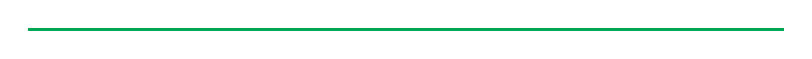
\begin{tikzpicture}
\fill[BOGreen] (0,0) rectangle (96mm,1.2pt);
\end{tikzpicture}\par\vspace{8pt}
{\Large\sffamily\bfseries\color{BONavy} Cost, return and timing will determine the real deployment window}\par\vspace{4pt}
{\sffamily\fontsize{15}{20}\selectfont\color{BOGreen} Market size should not enter an investment case until the cost and return logic can be checked.}\par\vspace{9pt}
\begin{multicols}{2}
{\small The board-level question is whether every opportunity eventually returns to cost, revenue, margin, cash flow and timing. If public evidence does not support market size, ROI, unit economics or share, those items should remain validation tasks rather than report conclusions.}\par
{\small For leadership teams, near-term action should focus on verifiable cost drivers and customer willingness to pay instead of relying on optimistic long-range scenarios. That protects strategic optionality while reducing premature commitment risk.}\par
{\small As cost, customer and financing evidence improves, management can shift resources from monitoring and partnerships toward pilots or scaled deployment.}\par
{\small For a CEO, Cost, return and timing will determine the real deployment window matters only if it changes the timing of capital, partner access, customer commitments or risk appetite. The strongest posture is to keep learning close to the business while reserving heavier commitments for proof that can survive investment-committee scrutiny.}\par
{\small For Cost, return and timing will determine the real deployment window, resource allocation should follow the facts that can change the decision: customer demand, cost position, financing availability, regulatory path and delivery capability. If those facts do not improve, increasing exposure mainly creates strategic lock-in rather than higher conviction.}\par
\end{multicols}
\label{chap:7:end}

\clearpage
{\textcolor{BOGreen}{\scriptsize\bfseries EXHIBIT 7}}\par\vspace{4pt}
{\sffamily\fontsize{17}{21}\selectfont\color{BONavy} Cost structure must be decomposed before underwriting}\par
{\small\color{BOText} Cost diligence view for Nuclear Fusion Commercialization: Strategic Implications for Energy Markets and Capital Allocation}\par\vspace{6pt}
\noindent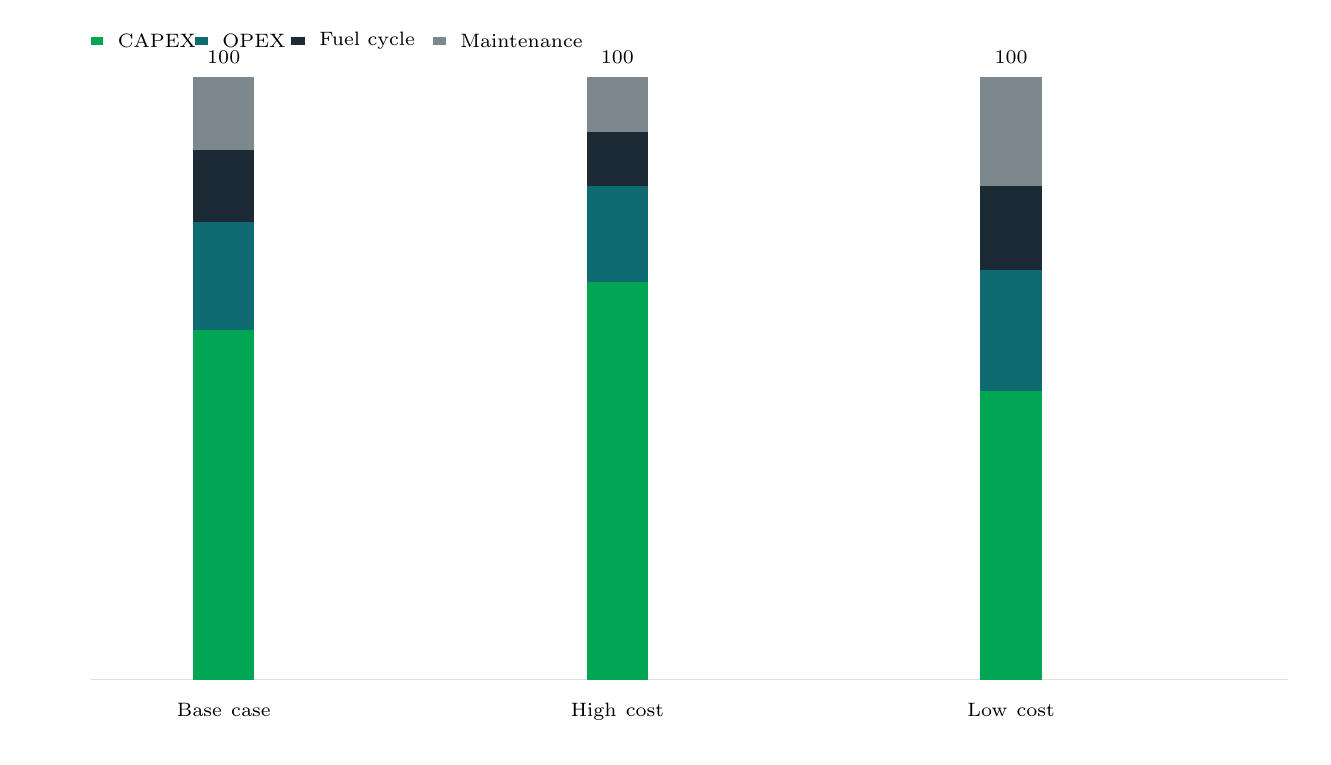
\begin{tikzpicture}[x=1cm,y=1cm]
\path[use as bounding box] (0,0) rectangle (16.20,9.00);
\draw[BOLine] (0.80,0.72) -- (16.00,0.72);
\fill[BOGreen] (2.10,0.72) rectangle (2.88,5.16);
\fill[BOBlue] (2.10,5.16) rectangle (2.88,6.53);
\fill[BONavy] (2.10,6.53) rectangle (2.88,7.45);
\fill[BOMuted] (2.10,7.45) rectangle (2.88,8.37);
\node[anchor=south,align=center] at (2.49,8.42) {\scriptsize 100};
\node[anchor=north,align=center,text width=4.60cm] at (2.49,0.55) {\scriptsize Base case};
\fill[BOGreen] (7.10,0.72) rectangle (7.88,5.77);
\fill[BOBlue] (7.10,5.77) rectangle (7.88,6.99);
\fill[BONavy] (7.10,6.99) rectangle (7.88,7.68);
\fill[BOMuted] (7.10,7.68) rectangle (7.88,8.37);
\node[anchor=south,align=center] at (7.49,8.42) {\scriptsize 100};
\node[anchor=north,align=center,text width=4.60cm] at (7.49,0.55) {\scriptsize High cost};
\fill[BOGreen] (12.10,0.72) rectangle (12.88,4.39);
\fill[BOBlue] (12.10,4.39) rectangle (12.88,5.92);
\fill[BONavy] (12.10,5.92) rectangle (12.88,6.99);
\fill[BOMuted] (12.10,6.99) rectangle (12.88,8.37);
\node[anchor=south,align=center] at (12.49,8.42) {\scriptsize 100};
\node[anchor=north,align=center,text width=4.60cm] at (12.49,0.55) {\scriptsize Low cost};
\fill[BOGreen] (0.80,8.78) rectangle (0.96,8.88);
\node[anchor=west] at (1.02,8.83) {\scriptsize CAPEX};
\fill[BOBlue] (2.12,8.78) rectangle (2.29,8.88);
\node[anchor=west] at (2.35,8.83) {\scriptsize OPEX};
\fill[BONavy] (3.35,8.78) rectangle (3.52,8.88);
\node[anchor=west] at (3.58,8.83) {\scriptsize Fuel cycle};
\fill[BOMuted] (5.15,8.78) rectangle (5.31,8.88);
\node[anchor=west] at (5.37,8.83) {\scriptsize Maintenance};
\end{tikzpicture}\par\vspace{2pt}
\vspace{3pt}\noindent\begin{minipage}[t]{0.58\linewidth}
\textcolor{BOGreen}{\rule{24mm}{0.6pt}}\par\vspace{3pt}
{\footnotesize\color{BOText} The chart separates capital, operating and maintenance drivers so management can test which cost lever would change the investment case.}\par\vspace{2pt}
{\footnotesize\color{BOText} Base case is the highest visible point at 100, while Base case sets the lower bound at 100.}\par\vspace{2pt}
\end{minipage}\hfill\begin{minipage}[t]{0.36\linewidth}
\vspace{1pt}{\scriptsize\color{BOText}\begin{tabular}{p{31mm}>{\raggedleft\arraybackslash}p{18mm}}
\multicolumn{2}{l}{\textcolor{BOGreen}{\bfseries Visible readout}}\\[2pt]
Base case & \textbf{100}\\[1pt]
High cost & \textbf{100}\\[1pt]
Low cost & \textbf{100}\\[1pt]
\end{tabular}}\par
\end{minipage}\par\vspace{2pt}
\vspace{4pt}{\footnotesize\color{BOText} The chart separates capital, operating and maintenance drivers so management can test which cost lever would change the investment case.}\par
{\scriptsize\color{BOMuted} BlueOcean public-source synthesis.}\par

\clearpage
\label{chap:8}
\noindent\begin{tikzpicture}
\path[use as bounding box] (0,0) rectangle (\linewidth,54mm);
\clip (0,0) rectangle (\linewidth,54mm);
\node[anchor=north west,inner sep=0] at (0,54mm) {
\includegraphics[width=\linewidth]{assets/image-8.png}};
\end{tikzpicture}
\vspace{0pt}
\noindent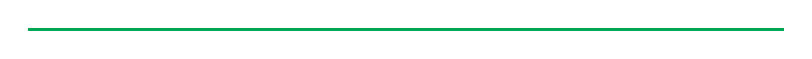
\begin{tikzpicture}
\fill[BOGreen] (0,0) rectangle (96mm,1.2pt);
\end{tikzpicture}\par\vspace{8pt}
{\Large\sffamily\bfseries\color{BONavy} Regulation, policy and public acceptance can reset the speed of adoption}\par\vspace{4pt}
{\sffamily\fontsize{15}{20}\selectfont\color{BOGreen} External rules can accelerate the market or change the risk budget and project timeline.}\par\vspace{9pt}
\begin{multicols}{2}
{\small For leadership teams, policy support, permitting rules, standards and public acceptance affect how quickly an opportunity moves from concept to deployment. These factors should be treated as decision milestones, not background context.}\par
{\small A practical reading is that where the regulatory path is unclear, the better move is usually standards engagement, policy tracking and low-risk pilots rather than an early heavy-asset commitment.}\par
{\small The decision lens is that the board should track which policy events would change investment timing, such as licensing rules, procurement requirements, subsidy treatment, local approvals or safety standards.}\par
{\small For capital allocation, for a CEO, Regulation, policy and public acceptance can reset the speed of adoption matters only if it changes the timing of capital, partner access, customer commitments or risk appetite. The strongest posture is to keep learning close to the business while reserving heavier commitments for proof that can survive investment-committee scrutiny.}\par
{\small For Regulation, policy and public acceptance can reset the speed of adoption, resource allocation should follow the facts that can change the decision: customer demand, cost position, financing availability, regulatory path and delivery capability. If those facts do not improve, increasing exposure mainly creates strategic lock-in rather than higher conviction.}\par
\end{multicols}
\label{chap:8:end}

\clearpage
{\textcolor{BOGreen}{\scriptsize\bfseries EXHIBIT 8}}\par\vspace{4pt}
{\sffamily\fontsize{17}{21}\selectfont\color{BONavy} Timeline confidence falls as milestones move from lab to grid}\par
{\small\color{BOText} Milestone confidence for Nuclear Fusion Commercialization: Strategic Implications for Energy Markets and Capital Allocation}\par\vspace{6pt}
\noindent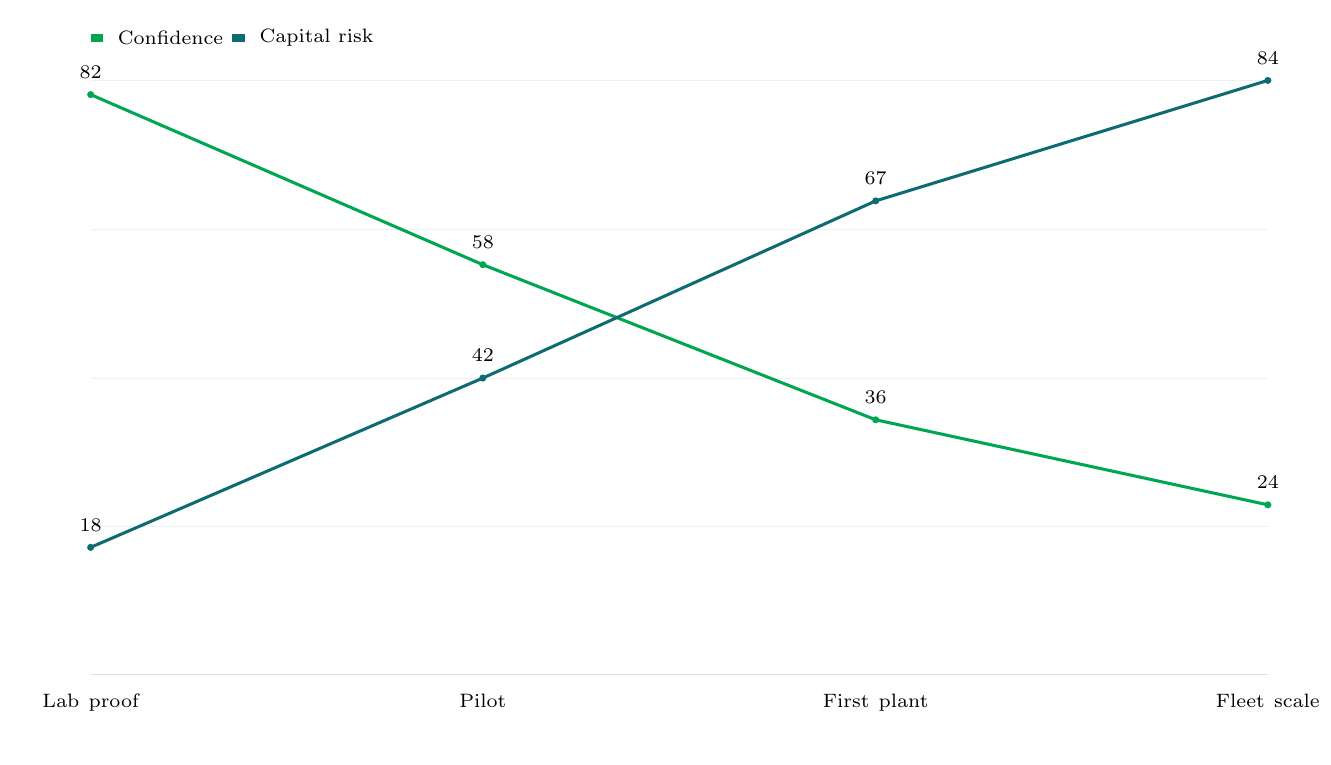
\begin{tikzpicture}[x=1cm,y=1cm]
\path[use as bounding box] (0,0) rectangle (16.20,9.00);
\draw[BOLine] (0.80,0.78) -- (15.75,0.78);
\draw[BOLine,opacity=.45] (0.80,2.67) -- (15.75,2.67);
\draw[BOLine,opacity=.45] (0.80,4.55) -- (15.75,4.55);
\draw[BOLine,opacity=.45] (0.80,6.44) -- (15.75,6.44);
\draw[BOLine,opacity=.45] (0.80,8.33) -- (15.75,8.33);
\draw[BOGreen,line width=1.1pt] (0.80,8.15) -- (5.78,5.99) -- (10.77,4.02) -- (15.75,2.94);
\fill[BOGreen] (0.80,8.15) circle (.045);
\node[anchor=south,align=center] at (0.80,8.23) {\scriptsize 82};
\fill[BOGreen] (5.78,5.99) circle (.045);
\node[anchor=south,align=center] at (5.78,6.07) {\scriptsize 58};
\fill[BOGreen] (10.77,4.02) circle (.045);
\node[anchor=south,align=center] at (10.77,4.10) {\scriptsize 36};
\fill[BOGreen] (15.75,2.94) circle (.045);
\node[anchor=south,align=center] at (15.75,3.02) {\scriptsize 24};
\draw[BOBlue,line width=1.1pt] (0.80,2.40) -- (5.78,4.55) -- (10.77,6.80) -- (15.75,8.33);
\fill[BOBlue] (0.80,2.40) circle (.045);
\node[anchor=south,align=center] at (0.80,2.48) {\scriptsize 18};
\fill[BOBlue] (5.78,4.55) circle (.045);
\node[anchor=south,align=center] at (5.78,4.63) {\scriptsize 42};
\fill[BOBlue] (10.77,6.80) circle (.045);
\node[anchor=south,align=center] at (10.77,6.88) {\scriptsize 67};
\fill[BOBlue] (15.75,8.33) circle (.045);
\node[anchor=south,align=center] at (15.75,8.41) {\scriptsize 84};
\node[anchor=north,align=center,text width=1.8cm] at (0.80,0.66) {\scriptsize Lab proof};
\node[anchor=north,align=center,text width=1.8cm] at (5.78,0.66) {\scriptsize Pilot};
\node[anchor=north,align=center,text width=1.8cm] at (10.77,0.66) {\scriptsize First plant};
\node[anchor=north,align=center,text width=1.8cm] at (15.75,0.66) {\scriptsize Fleet scale};
\fill[BOGreen] (0.80,8.82) rectangle (0.96,8.92);
\node[anchor=west] at (1.02,8.87) {\scriptsize Confidence};
\fill[BOBlue] (2.60,8.82) rectangle (2.76,8.92);
\node[anchor=west] at (2.82,8.87) {\scriptsize Capital risk};
\end{tikzpicture}\par\vspace{2pt}
\vspace{3pt}\noindent\begin{minipage}[t]{0.58\linewidth}
\textcolor{BOGreen}{\rule{24mm}{0.6pt}}\par\vspace{3pt}
{\footnotesize\color{BOText} Decision confidence should be staged by milestone maturity.}\par\vspace{2pt}
{\footnotesize\color{BOText} Fleet scale is the highest visible point at 108, while Lab proof sets the lower bound at 100.}\par\vspace{2pt}
\end{minipage}\hfill\begin{minipage}[t]{0.36\linewidth}
\vspace{1pt}{\scriptsize\color{BOText}\begin{tabular}{p{31mm}>{\raggedleft\arraybackslash}p{18mm}}
\multicolumn{2}{l}{\textcolor{BOGreen}{\bfseries Visible readout}}\\[2pt]
Lab proof & \textbf{100}\\[1pt]
Pilot & \textbf{100}\\[1pt]
First plant & \textbf{103}\\[1pt]
Fleet scale & \textbf{108}\\[1pt]
\end{tabular}}\par
\end{minipage}\par\vspace{2pt}
\vspace{4pt}{\footnotesize\color{BOText} Decision confidence should be staged by milestone maturity.}\par
{\scriptsize\color{BOMuted} BlueOcean milestone assessment.}\par

\clearpage
{\textcolor{BOGreen}{\scriptsize\bfseries EXHIBIT 9}}\par\vspace{4pt}
{\sffamily\fontsize{17}{21}\selectfont\color{BONavy} Partner options differ on learning value and capital exposure}\par
{\small\color{BOText} Where-to-play option view for Nuclear Fusion Commercialization: Strategic Implications for Energy Markets and Capital Allocation}\par\vspace{6pt}
{\scriptsize\begin{tabular}{p{38mm}>{\centering\arraybackslash}p{21mm}>{\centering\arraybackslash}p{21mm}>{\centering\arraybackslash}p{21mm}>{\centering\arraybackslash}p{21mm}}
 & {\bfseries Learning} & {\bfseries Control} & {\bfseries Capital need} & {\bfseries Reversibility} \\
\hline
{\bfseries Direct equity} & \colorbox{BOGreen}{\textcolor{white}{\strut\hspace{5pt}5\hspace{5pt}}} & \colorbox{BOGreen}{\textcolor{white}{\strut\hspace{5pt}4\hspace{5pt}}} & \colorbox{BOLight}{\textcolor{BOText}{\strut\hspace{5pt}2\hspace{5pt}}} & \colorbox{BOLight}{\textcolor{BOText}{\strut\hspace{5pt}2\hspace{5pt}}} \\
{\bfseries Corporate venture} & \colorbox{BOGreen}{\textcolor{white}{\strut\hspace{5pt}4\hspace{5pt}}} & \colorbox{BOBlue}{\textcolor{white}{\strut\hspace{5pt}3\hspace{5pt}}} & \colorbox{BOBlue}{\textcolor{white}{\strut\hspace{5pt}3\hspace{5pt}}} & \colorbox{BOBlue}{\textcolor{white}{\strut\hspace{5pt}3\hspace{5pt}}} \\
{\bfseries Offtake option} & \colorbox{BOBlue}{\textcolor{white}{\strut\hspace{5pt}3\hspace{5pt}}} & \colorbox{BOLight}{\textcolor{BOText}{\strut\hspace{5pt}2\hspace{5pt}}} & \colorbox{BOGreen}{\textcolor{white}{\strut\hspace{5pt}4\hspace{5pt}}} & \colorbox{BOGreen}{\textcolor{white}{\strut\hspace{5pt}4\hspace{5pt}}} \\
{\bfseries Supplier JV} & \colorbox{BOGreen}{\textcolor{white}{\strut\hspace{5pt}4\hspace{5pt}}} & \colorbox{BOGreen}{\textcolor{white}{\strut\hspace{5pt}4\hspace{5pt}}} & \colorbox{BOLight}{\textcolor{BOText}{\strut\hspace{5pt}2\hspace{5pt}}} & \colorbox{BOLight}{\textcolor{BOText}{\strut\hspace{5pt}2\hspace{5pt}}} \\
{\bfseries R\&D consortium} & \colorbox{BOBlue}{\textcolor{white}{\strut\hspace{5pt}3\hspace{5pt}}} & \colorbox{BOLight}{\textcolor{BOText}{\strut\hspace{5pt}2\hspace{5pt}}} & \colorbox{BOGreen}{\textcolor{white}{\strut\hspace{5pt}5\hspace{5pt}}} & \colorbox{BOGreen}{\textcolor{white}{\strut\hspace{5pt}5\hspace{5pt}}} \\
\end{tabular}}\par\vspace{2pt}
\vspace{3pt}\noindent\begin{minipage}[t]{0.58\linewidth}
\textcolor{BOGreen}{\rule{24mm}{0.6pt}}\par\vspace{3pt}
{\footnotesize\color{BOText} The best early posture maximizes learning without forcing irreversible capital exposure.}\par\vspace{2pt}
{\footnotesize\color{BOText} The matrix compares 5 options across Learning, Control, Capital need, which keeps the page focused on relative choices rather than a single score.}\par\vspace{2pt}
\end{minipage}\hfill\begin{minipage}[t]{0.36\linewidth}
\vspace{1pt}{\scriptsize\color{BOText}\begin{tabular}{p{31mm}>{\raggedleft\arraybackslash}p{18mm}}
\multicolumn{2}{l}{\textcolor{BOGreen}{\bfseries Matrix readout}}\\[2pt]
Direct equity & \textbf{5 / 4}\\[1pt]
Corporate venture & \textbf{4 / 3}\\[1pt]
Offtake option & \textbf{3 / 2}\\[1pt]
Supplier JV & \textbf{4 / 4}\\[1pt]
\end{tabular}}\par
\end{minipage}\par\vspace{2pt}
\vspace{4pt}{\footnotesize\color{BOText} The best early posture maximizes learning without forcing irreversible capital exposure.}\par
{\scriptsize\color{BOMuted} BlueOcean option synthesis.}\par

\clearpage
{\textcolor{BOGreen}{\scriptsize\bfseries EXHIBIT 10}}\par\vspace{4pt}
{\sffamily\fontsize{17}{21}\selectfont\color{BONavy} Evidence maturity varies sharply by claim type}\par
{\small\color{BOText} Claim maturity for Nuclear Fusion Commercialization: Strategic Implications for Energy Markets and Capital Allocation}\par\vspace{6pt}
\noindent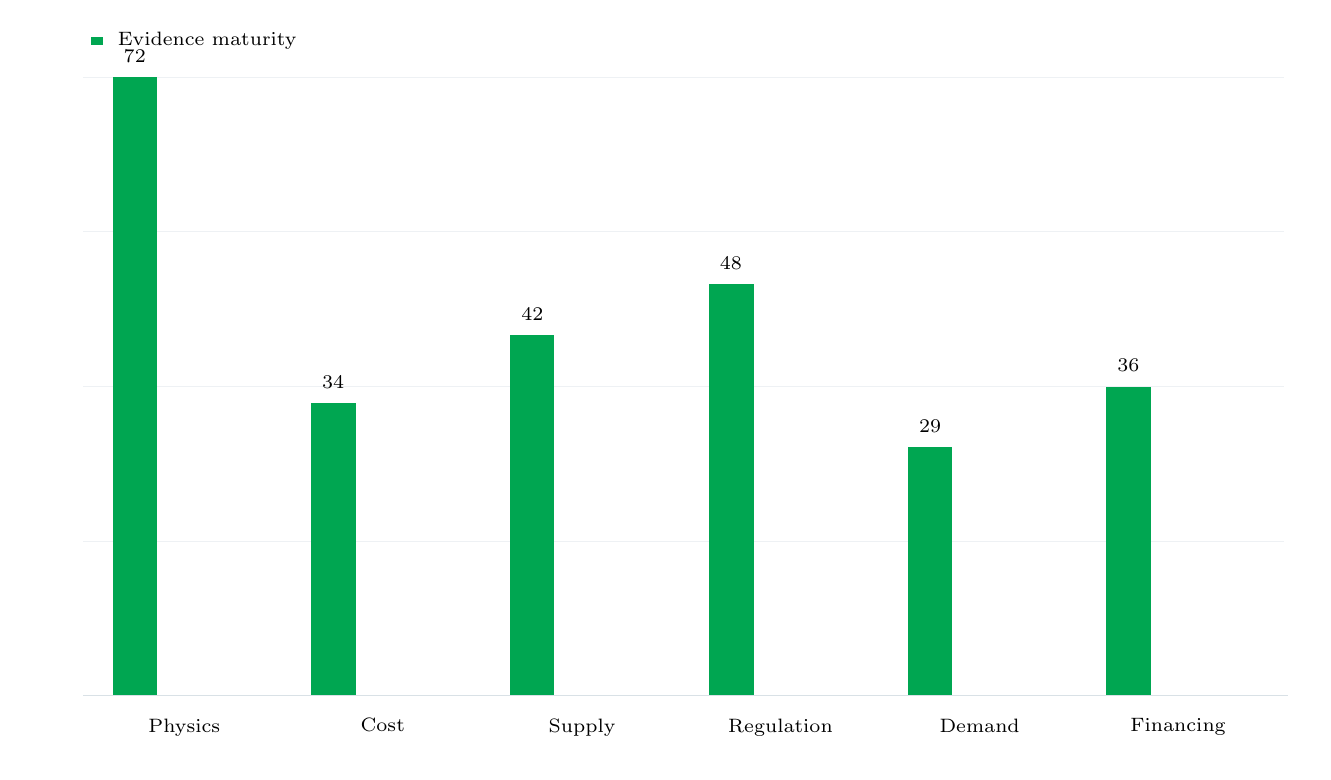
\begin{tikzpicture}[x=1cm,y=1cm]
\path[use as bounding box] (0,0) rectangle (16.20,9.20);
\draw[BOLine] (0.70,0.72) -- (16.00,0.72);
\draw[BOLine,opacity=.45] (0.70,2.68) -- (15.95,2.68);
\draw[BOLine,opacity=.45] (0.70,4.64) -- (15.95,4.64);
\draw[BOLine,opacity=.45] (0.70,6.61) -- (15.95,6.61);
\draw[BOLine,opacity=.45] (0.70,8.57) -- (15.95,8.57);
\fill[BOGreen] (1.08,0.72) rectangle (1.64,8.57);
\node[anchor=south,align=center] at (1.36,8.63) {\scriptsize 72};
\node[anchor=north,align=center,text width=2.32cm] at (1.99,0.55) {\scriptsize Physics};
\fill[BOGreen] (3.60,0.72) rectangle (4.17,4.43);
\node[anchor=south,align=center] at (3.88,4.49) {\scriptsize 34};
\node[anchor=north,align=center,text width=2.32cm] at (4.51,0.55) {\scriptsize Cost};
\fill[BOGreen] (6.13,0.72) rectangle (6.69,5.30);
\node[anchor=south,align=center] at (6.41,5.36) {\scriptsize 42};
\node[anchor=north,align=center,text width=2.32cm] at (7.04,0.55) {\scriptsize Supply};
\fill[BOGreen] (8.65,0.72) rectangle (9.22,5.95);
\node[anchor=south,align=center] at (8.93,6.01) {\scriptsize 48};
\node[anchor=north,align=center,text width=2.32cm] at (9.56,0.55) {\scriptsize Regulation};
\fill[BOGreen] (11.18,0.72) rectangle (11.74,3.88);
\node[anchor=south,align=center] at (11.46,3.94) {\scriptsize 29};
\node[anchor=north,align=center,text width=2.32cm] at (12.09,0.55) {\scriptsize Demand};
\fill[BOGreen] (13.70,0.72) rectangle (14.27,4.64);
\node[anchor=south,align=center] at (13.98,4.71) {\scriptsize 36};
\node[anchor=north,align=center,text width=2.32cm] at (14.61,0.55) {\scriptsize Financing};
\fill[BOGreen] (0.80,8.98) rectangle (0.96,9.08);
\node[anchor=west] at (1.02,9.03) {\scriptsize Evidence maturity};
\end{tikzpicture}\par\vspace{2pt}
\vspace{3pt}\noindent\begin{minipage}[t]{0.58\linewidth}
\textcolor{BOGreen}{\rule{24mm}{0.6pt}}\par\vspace{3pt}
{\footnotesize\color{BOText} Management can use the maturity gap to decide which claims support action today and which require a separate diligence workstream.}\par\vspace{2pt}
{\footnotesize\color{BOText} Physics is the highest visible point at 72, while Demand sets the lower bound at 29.}\par\vspace{2pt}
\end{minipage}\hfill\begin{minipage}[t]{0.36\linewidth}
\vspace{1pt}{\scriptsize\color{BOText}\begin{tabular}{p{31mm}>{\raggedleft\arraybackslash}p{18mm}}
\multicolumn{2}{l}{\textcolor{BOGreen}{\bfseries Visible readout}}\\[2pt]
Physics & \textbf{72}\\[1pt]
Cost & \textbf{34}\\[1pt]
Supply & \textbf{42}\\[1pt]
Regulation & \textbf{48}\\[1pt]
Demand & \textbf{29}\\[1pt]
\end{tabular}}\par
\end{minipage}\par\vspace{2pt}
\vspace{4pt}{\footnotesize\color{BOText} Management can use the maturity gap to decide which claims support action today and which require a separate diligence workstream.}\par
{\scriptsize\color{BOMuted} BlueOcean public-source synthesis.}\par

\clearpage
{\textcolor{BOGreen}{\scriptsize\bfseries EXHIBIT 11}}\par\vspace{4pt}
{\sffamily\fontsize{17}{21}\selectfont\color{BONavy} Use-case priorities separate early revenue from long-term optionality}\par
{\small\color{BOText} Customer option screen for Nuclear Fusion Commercialization: Strategic Implications for Energy Markets and Capital Allocation}\par\vspace{6pt}
{\scriptsize\begin{tabular}{p{38mm}>{\centering\arraybackslash}p{21mm}>{\centering\arraybackslash}p{21mm}>{\centering\arraybackslash}p{21mm}>{\centering\arraybackslash}p{21mm}}
 & {\bfseries Demand pull} & {\bfseries Price tolerance} & {\bfseries Timing} & {\bfseries Evidence} \\
\hline
{\bfseries Industrial heat} & \colorbox{BOGreen}{\textcolor{white}{\strut\hspace{5pt}5\hspace{5pt}}} & \colorbox{BOGreen}{\textcolor{white}{\strut\hspace{5pt}4\hspace{5pt}}} & \colorbox{BOBlue}{\textcolor{white}{\strut\hspace{5pt}3\hspace{5pt}}} & \colorbox{BOBlue}{\textcolor{white}{\strut\hspace{5pt}3\hspace{5pt}}} \\
{\bfseries Hydrogen} & \colorbox{BOGreen}{\textcolor{white}{\strut\hspace{5pt}4\hspace{5pt}}} & \colorbox{BOGreen}{\textcolor{white}{\strut\hspace{5pt}4\hspace{5pt}}} & \colorbox{BOBlue}{\textcolor{white}{\strut\hspace{5pt}3\hspace{5pt}}} & \colorbox{BOLight}{\textcolor{BOText}{\strut\hspace{5pt}2\hspace{5pt}}} \\
{\bfseries Grid power} & \colorbox{BOGreen}{\textcolor{white}{\strut\hspace{5pt}5\hspace{5pt}}} & \colorbox{BOLight}{\textcolor{BOText}{\strut\hspace{5pt}2\hspace{5pt}}} & \colorbox{BOLight}{\textcolor{BOText}{\strut\hspace{5pt}1\hspace{5pt}}} & \colorbox{BOLight}{\textcolor{BOText}{\strut\hspace{5pt}2\hspace{5pt}}} \\
{\bfseries Defense / remote} & \colorbox{BOBlue}{\textcolor{white}{\strut\hspace{5pt}3\hspace{5pt}}} & \colorbox{BOGreen}{\textcolor{white}{\strut\hspace{5pt}5\hspace{5pt}}} & \colorbox{BOBlue}{\textcolor{white}{\strut\hspace{5pt}3\hspace{5pt}}} & \colorbox{BOLight}{\textcolor{BOText}{\strut\hspace{5pt}2\hspace{5pt}}} \\
{\bfseries Research services} & \colorbox{BOLight}{\textcolor{BOText}{\strut\hspace{5pt}2\hspace{5pt}}} & \colorbox{BOBlue}{\textcolor{white}{\strut\hspace{5pt}3\hspace{5pt}}} & \colorbox{BOGreen}{\textcolor{white}{\strut\hspace{5pt}4\hspace{5pt}}} & \colorbox{BOGreen}{\textcolor{white}{\strut\hspace{5pt}4\hspace{5pt}}} \\
\end{tabular}}\par\vspace{2pt}
\vspace{3pt}\noindent\begin{minipage}[t]{0.58\linewidth}
\textcolor{BOGreen}{\rule{24mm}{0.6pt}}\par\vspace{3pt}
{\footnotesize\color{BOText} The comparison separates markets that can teach the company soon from markets that may require longer proof cycles.}\par\vspace{2pt}
{\footnotesize\color{BOText} The matrix compares 5 options across Demand pull, Price tolerance, Timing, which keeps the page focused on relative choices rather than a single score.}\par\vspace{2pt}
\end{minipage}\hfill\begin{minipage}[t]{0.36\linewidth}
\vspace{1pt}{\scriptsize\color{BOText}\begin{tabular}{p{31mm}>{\raggedleft\arraybackslash}p{18mm}}
\multicolumn{2}{l}{\textcolor{BOGreen}{\bfseries Matrix readout}}\\[2pt]
Industrial heat & \textbf{5 / 4}\\[1pt]
Hydrogen & \textbf{4 / 4}\\[1pt]
Grid power & \textbf{5 / 2}\\[1pt]
Defense / remote & \textbf{3 / 5}\\[1pt]
\end{tabular}}\par
\end{minipage}\par\vspace{2pt}
\vspace{4pt}{\footnotesize\color{BOText} The comparison separates markets that can teach the company soon from markets that may require longer proof cycles.}\par
{\scriptsize\color{BOMuted} BlueOcean customer option synthesis.}\par

\clearpage
{\textcolor{BOGreen}{\scriptsize\bfseries EXHIBIT 12}}\par\vspace{4pt}
{\sffamily\fontsize{17}{21}\selectfont\color{BONavy} Capital exposure should be staged by decision milestone}\par
{\small\color{BOText} Commitment profile for Nuclear Fusion Commercialization: Strategic Implications for Energy Markets and Capital Allocation}\par\vspace{6pt}
\noindent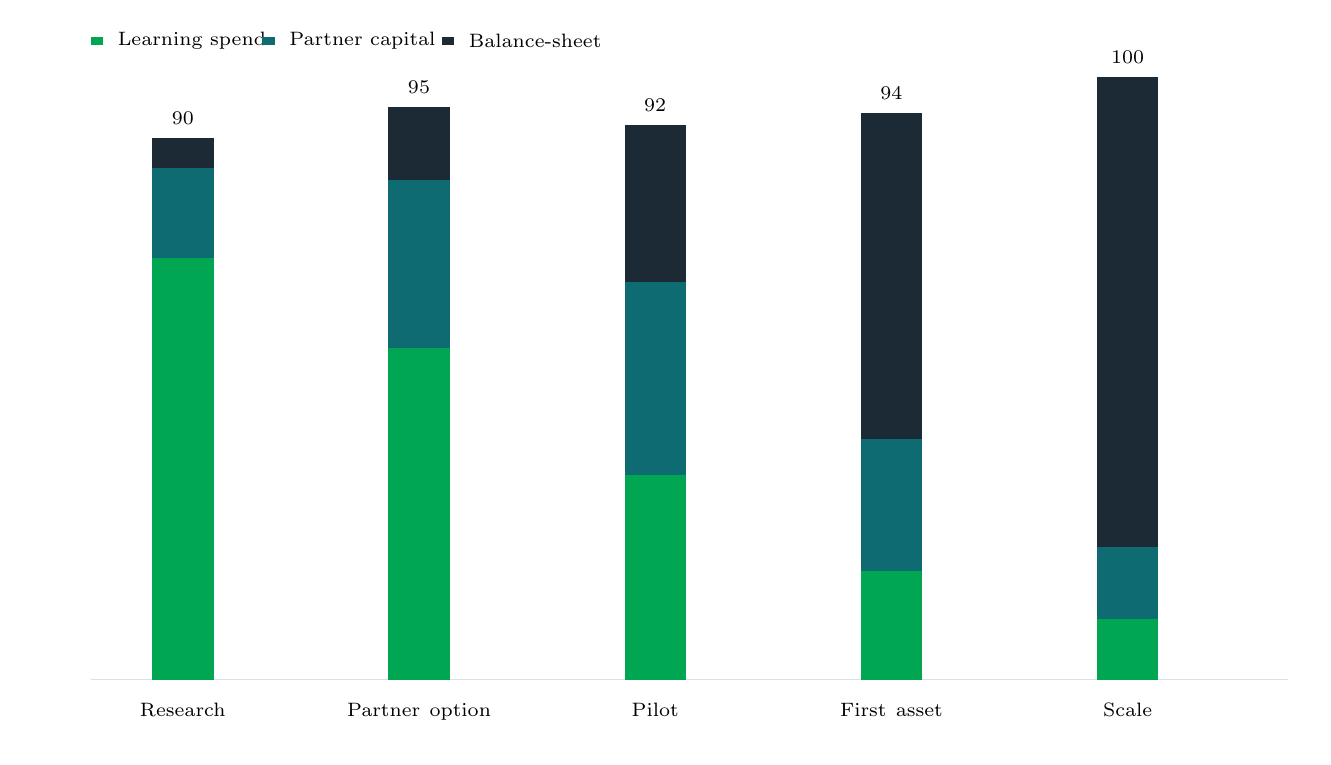
\begin{tikzpicture}[x=1cm,y=1cm]
\path[use as bounding box] (0,0) rectangle (16.20,9.00);
\draw[BOLine] (0.80,0.72) -- (16.00,0.72);
\fill[BOGreen] (1.58,0.72) rectangle (2.36,6.07);
\fill[BOBlue] (1.58,6.07) rectangle (2.36,7.22);
\fill[BONavy] (1.58,7.22) rectangle (2.36,7.60);
\node[anchor=south,align=center] at (1.97,7.65) {\scriptsize 90};
\node[anchor=north,align=center,text width=2.76cm] at (1.97,0.55) {\scriptsize Research};
\fill[BOGreen] (4.58,0.72) rectangle (5.36,4.93);
\fill[BOBlue] (4.58,4.93) rectangle (5.36,7.07);
\fill[BONavy] (4.58,7.07) rectangle (5.36,7.99);
\node[anchor=south,align=center] at (4.97,8.04) {\scriptsize 95};
\node[anchor=north,align=center,text width=2.76cm] at (4.97,0.55) {\scriptsize Partner option};
\fill[BOGreen] (7.58,0.72) rectangle (8.36,3.32);
\fill[BOBlue] (7.58,3.32) rectangle (8.36,5.77);
\fill[BONavy] (7.58,5.77) rectangle (8.36,7.76);
\node[anchor=south,align=center] at (7.97,7.81) {\scriptsize 92};
\node[anchor=north,align=center,text width=2.76cm] at (7.97,0.55) {\scriptsize Pilot};
\fill[BOGreen] (10.58,0.72) rectangle (11.36,2.10);
\fill[BOBlue] (10.58,2.10) rectangle (11.36,3.78);
\fill[BONavy] (10.58,3.78) rectangle (11.36,7.91);
\node[anchor=south,align=center] at (10.97,7.96) {\scriptsize 94};
\node[anchor=north,align=center,text width=2.76cm] at (10.97,0.55) {\scriptsize First asset};
\fill[BOGreen] (13.58,0.72) rectangle (14.36,1.49);
\fill[BOBlue] (13.58,1.49) rectangle (14.36,2.40);
\fill[BONavy] (13.58,2.40) rectangle (14.36,8.37);
\node[anchor=south,align=center] at (13.97,8.42) {\scriptsize 100};
\node[anchor=north,align=center,text width=2.76cm] at (13.97,0.55) {\scriptsize Scale};
\fill[BOGreen] (0.80,8.78) rectangle (0.96,8.88);
\node[anchor=west] at (1.02,8.83) {\scriptsize Learning spend};
\fill[BOBlue] (2.98,8.78) rectangle (3.14,8.88);
\node[anchor=west] at (3.20,8.83) {\scriptsize Partner capital};
\fill[BONavy] (5.26,8.78) rectangle (5.42,8.88);
\node[anchor=west] at (5.48,8.83) {\scriptsize Balance-sheet};
\end{tikzpicture}\par\vspace{2pt}
\vspace{3pt}\noindent\begin{minipage}[t]{0.58\linewidth}
\textcolor{BOGreen}{\rule{24mm}{0.6pt}}\par\vspace{3pt}
{\footnotesize\color{BOText} The capital mix should move from learning to committed exposure only as evidence matures.}\par\vspace{2pt}
{\footnotesize\color{BOText} Scale is the highest visible point at 100, while Research sets the lower bound at 90.}\par\vspace{2pt}
\end{minipage}\hfill\begin{minipage}[t]{0.36\linewidth}
\vspace{1pt}{\scriptsize\color{BOText}\begin{tabular}{p{31mm}>{\raggedleft\arraybackslash}p{18mm}}
\multicolumn{2}{l}{\textcolor{BOGreen}{\bfseries Visible readout}}\\[2pt]
Research & \textbf{90}\\[1pt]
Partner option & \textbf{95}\\[1pt]
Pilot & \textbf{92}\\[1pt]
First asset & \textbf{94}\\[1pt]
Scale & \textbf{100}\\[1pt]
\end{tabular}}\par
\end{minipage}\par\vspace{2pt}
\vspace{4pt}{\footnotesize\color{BOText} The capital mix should move from learning to committed exposure only as evidence matures.}\par
{\scriptsize\color{BOMuted} BlueOcean capital staging view.}\par

\clearpage
{\textcolor{BOGreen}{\scriptsize\bfseries EXHIBIT 13}}\par\vspace{4pt}
{\sffamily\fontsize{17}{21}\selectfont\color{BONavy} Management attention shifts as the uncertainty stack resolves}\par
{\small\color{BOText} Executive review cadence for Nuclear Fusion Commercialization: Strategic Implications for Energy Markets and Capital Allocation}\par\vspace{6pt}
\noindent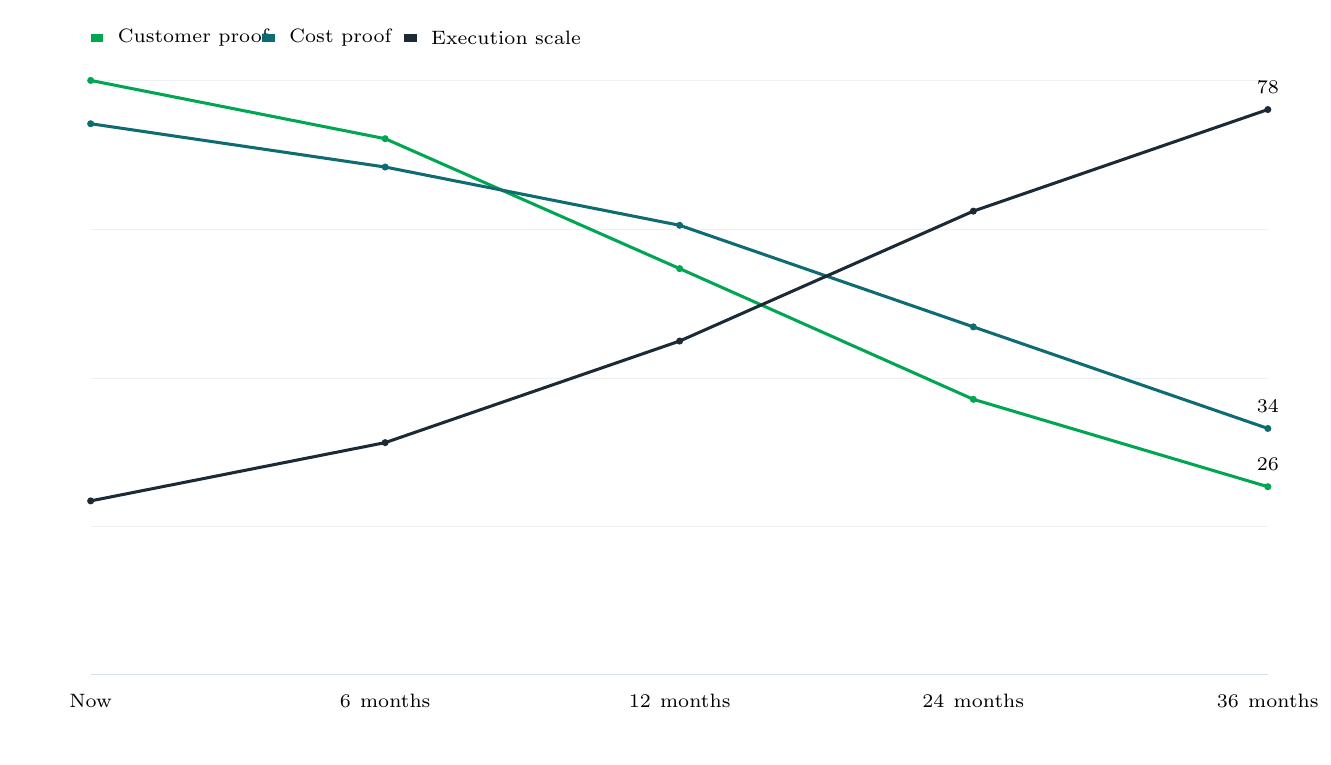
\begin{tikzpicture}[x=1cm,y=1cm]
\path[use as bounding box] (0,0) rectangle (16.20,9.00);
\draw[BOLine] (0.80,0.78) -- (15.75,0.78);
\draw[BOLine,opacity=.45] (0.80,2.67) -- (15.75,2.67);
\draw[BOLine,opacity=.45] (0.80,4.55) -- (15.75,4.55);
\draw[BOLine,opacity=.45] (0.80,6.44) -- (15.75,6.44);
\draw[BOLine,opacity=.45] (0.80,8.33) -- (15.75,8.33);
\draw[BOGreen,line width=1.1pt] (0.80,8.33) -- (4.54,7.59) -- (8.28,5.94) -- (12.01,4.28) -- (15.75,3.17);
\fill[BOGreen] (0.80,8.33) circle (.045);
\fill[BOGreen] (4.54,7.59) circle (.045);
\fill[BOGreen] (8.28,5.94) circle (.045);
\fill[BOGreen] (12.01,4.28) circle (.045);
\fill[BOGreen] (15.75,3.17) circle (.045);
\node[anchor=south,align=center] at (15.75,3.25) {\scriptsize 26};
\draw[BOBlue,line width=1.1pt] (0.80,7.78) -- (4.54,7.23) -- (8.28,6.49) -- (12.01,5.20) -- (15.75,3.91);
\fill[BOBlue] (0.80,7.78) circle (.045);
\fill[BOBlue] (4.54,7.23) circle (.045);
\fill[BOBlue] (8.28,6.49) circle (.045);
\fill[BOBlue] (12.01,5.20) circle (.045);
\fill[BOBlue] (15.75,3.91) circle (.045);
\node[anchor=south,align=center] at (15.75,3.99) {\scriptsize 34};
\draw[BONavy,line width=1.1pt] (0.80,2.99) -- (4.54,3.73) -- (8.28,5.02) -- (12.01,6.67) -- (15.75,7.96);
\fill[BONavy] (0.80,2.99) circle (.045);
\fill[BONavy] (4.54,3.73) circle (.045);
\fill[BONavy] (8.28,5.02) circle (.045);
\fill[BONavy] (12.01,6.67) circle (.045);
\fill[BONavy] (15.75,7.96) circle (.045);
\node[anchor=south,align=center] at (15.75,8.04) {\scriptsize 78};
\node[anchor=north,align=center,text width=1.8cm] at (0.80,0.66) {\scriptsize Now};
\node[anchor=north,align=center,text width=1.8cm] at (4.54,0.66) {\scriptsize 6 months};
\node[anchor=north,align=center,text width=1.8cm] at (8.28,0.66) {\scriptsize 12 months};
\node[anchor=north,align=center,text width=1.8cm] at (12.01,0.66) {\scriptsize 24 months};
\node[anchor=north,align=center,text width=1.8cm] at (15.75,0.66) {\scriptsize 36 months};
\fill[BOGreen] (0.80,8.82) rectangle (0.96,8.92);
\node[anchor=west] at (1.02,8.87) {\scriptsize Customer proof};
\fill[BOBlue] (2.98,8.82) rectangle (3.14,8.92);
\node[anchor=west] at (3.20,8.87) {\scriptsize Cost proof};
\fill[BONavy] (4.78,8.82) rectangle (4.94,8.92);
\node[anchor=west] at (5.00,8.87) {\scriptsize Execution scale};
\end{tikzpicture}\par\vspace{2pt}
\vspace{3pt}\noindent\begin{minipage}[t]{0.58\linewidth}
\textcolor{BOGreen}{\rule{24mm}{0.6pt}}\par\vspace{3pt}
{\footnotesize\color{BOText} The review agenda should shift from proof gathering toward scaling questions only after the earlier uncertainties narrow.}\par\vspace{2pt}
{\footnotesize\color{BOText} Now is the highest visible point at 182, while 36 months sets the lower bound at 138.}\par\vspace{2pt}
\end{minipage}\hfill\begin{minipage}[t]{0.36\linewidth}
\vspace{1pt}{\scriptsize\color{BOText}\begin{tabular}{p{31mm}>{\raggedleft\arraybackslash}p{18mm}}
\multicolumn{2}{l}{\textcolor{BOGreen}{\bfseries Visible readout}}\\[2pt]
Now & \textbf{182}\\[1pt]
6 months & \textbf{176}\\[1pt]
12 months & \textbf{164}\\[1pt]
24 months & \textbf{150}\\[1pt]
36 months & \textbf{138}\\[1pt]
\end{tabular}}\par
\end{minipage}\par\vspace{2pt}
\vspace{4pt}{\footnotesize\color{BOText} The review agenda should shift from proof gathering toward scaling questions only after the earlier uncertainties narrow.}\par
{\scriptsize\color{BOMuted} BlueOcean uncertainty-resolution model.}\par

\clearpage
{\textcolor{BOGreen}{\scriptsize\bfseries EXHIBIT 14}}\par\vspace{4pt}
{\sffamily\fontsize{17}{21}\selectfont\color{BONavy} Competitive posture depends on timing, access and reversibility}\par
{\small\color{BOText} Strategic posture map for Nuclear Fusion Commercialization: Strategic Implications for Energy Markets and Capital Allocation}\par\vspace{6pt}
\noindent\begin{tikzpicture}[x=1cm,y=1cm]
\path[use as bounding box] (0,0) rectangle (15.60,6.60);
\draw[BOLine] (0.85,0.65) -- (15.10,0.65) -- (15.10,6.00);
\draw[BOLine,dashed] (0.85,3.32) -- (15.10,3.32);
\draw[BOLine,dashed] (7.97,0.65) -- (7.97,6.00);
\fill[BOGreen,opacity=.65] (11.96,4.18) circle (0.20);
\node[anchor=east,align=right,text width=2.55cm] at (11.59,4.21) {\scriptsize Minority option};
\fill[BOGreen,opacity=.65] (10.54,4.61) circle (0.21);
\node[anchor=west,align=left,text width=2.55cm] at (10.93,4.82) {\scriptsize Offtake rights};
\fill[BOGreen,opacity=.65] (8.54,3.97) circle (0.18);
\node[anchor=west,align=left,text width=2.55cm] at (8.91,3.81) {\scriptsize Supplier JV};
\fill[BOGreen,opacity=.65] (6.26,5.04) circle (0.24);
\node[anchor=west,align=left,text width=2.55cm] at (6.68,5.43) {\scriptsize Direct build};
\fill[BOGreen,opacity=.65] (11.11,2.90) circle (0.16);
\node[anchor=east,align=right,text width=2.55cm] at (10.77,2.56) {\scriptsize Research consortium};
\node[anchor=north east] at (15.10,0.53) {\scriptsize Reversibility};
\node[anchor=center,rotate=90] at (0.55,3.32) {\scriptsize Strategic access};
\end{tikzpicture}\par\vspace{2pt}
\vspace{3pt}\noindent\begin{minipage}[t]{0.58\linewidth}
\textcolor{BOGreen}{\rule{24mm}{0.6pt}}\par\vspace{3pt}
{\footnotesize\color{BOText} Early moves should protect access and learning while avoiding positions that cannot be reversed if evidence weakens.}\par\vspace{2pt}
{\footnotesize\color{BOText} Minority option carries the strongest combined access and risk signal in the exhibit.}\par\vspace{2pt}
\end{minipage}\hfill\begin{minipage}[t]{0.36\linewidth}
\vspace{1pt}{\scriptsize\color{BOText}\begin{tabular}{p{31mm}>{\raggedleft\arraybackslash}p{18mm}}
\multicolumn{2}{l}{\textcolor{BOGreen}{\bfseries Position}}\\[2pt]
Minority option & \textbf{78 / 66}\\[1pt]
Offtake rights & \textbf{68 / 74}\\[1pt]
Supplier JV & \textbf{54 / 62}\\[1pt]
Direct build & \textbf{38 / 82}\\[1pt]
Research consortium & \textbf{72 / 42}\\[1pt]
\end{tabular}}\par
\end{minipage}\par\vspace{2pt}
\vspace{4pt}{\footnotesize\color{BOText} Early moves should protect access and learning while avoiding positions that cannot be reversed if evidence weakens.}\par
{\scriptsize\color{BOMuted} BlueOcean competitive posture screen.}\par

\clearpage
{\sffamily\fontsize{20}{25}\selectfont\color{BONavy} About the research}\par\vspace{6pt}
\vspace{2pt}{\color{BOBright}\rule{\linewidth}{1pt}}\vspace{5pt}
{\footnotesize\color{BOMuted} This report has been prepared for strategy discussion and executive decision support. It is not investment, legal, tax, audit or valuation advice. Market estimates, forecasts and scenarios are directional and should be independently validated before they are used for investment, financing, transaction, regulatory or operational decisions. Forward-looking views may change as technology, policy, financing, regulation, competition, supply chains and macro conditions evolve. Recipients should perform their own diligence and treat this report as one input into a broader decision process.}


\clearpage
\thispagestyle{empty}
\begin{tikzpicture}[remember picture,overlay]
\node[anchor=south west,inner sep=0] at (current page.south west) {
\includegraphics[width=\paperwidth,height=\paperheight]{assets/cover-ai.png}};
\fill[black,opacity=.45] (current page.south west) rectangle (current page.north east);
\node[anchor=south east] at ([xshift=-11mm,yshift=10mm]current page.south east) {\sffamily\bfseries\Large\color{white} BlueOcean};
\end{tikzpicture}

\end{document}
